\chapter{Applications of Differentiation}

\section{Tangent and Normal Lines}

In the previous chapter, we have learnt that the gradient of the tangent to the
curve $y=f(x)$ at point $P\big(x_0, f(x_0)\big)$ is
\begin{flalign*}
    m & = \lim_{\Delta x \to 0}\dfrac{f(x_0 + \Delta x) - f(x_0)}{\Delta x} & \\
      & = f'(x_0)
\end{flalign*}

\begin{multicols}{2}
    Hence, in order to find the tangent to the curve $y = f(x)$ at $x = x_0$, we just have to find the derivative value $f'(x_0)$ of the curve $y = f(x)$ at $x = x_0$, then the equation of the tangent line can be acquired through the point gradient formula of linear equations.

    As shown in the right figure, the line that passes through point $P$ and
    perpendicular to the tangent line $PT$ is known as the normal line to the curve
    $y = f(x)$. If two straight lines are perpendicular, the product of their
    gradients is $-1$. Since the gradient of the curve $y = f(x)$ at point $x =
        x_0$ is $f'(x_0)$, therefore when $f'(x_0) \neq 0$, the gradient of normal at
    point $x = x_0$ is $-\dfrac{1}{f'(x_0)}$.

    \columnbreak
    \begin{center}
        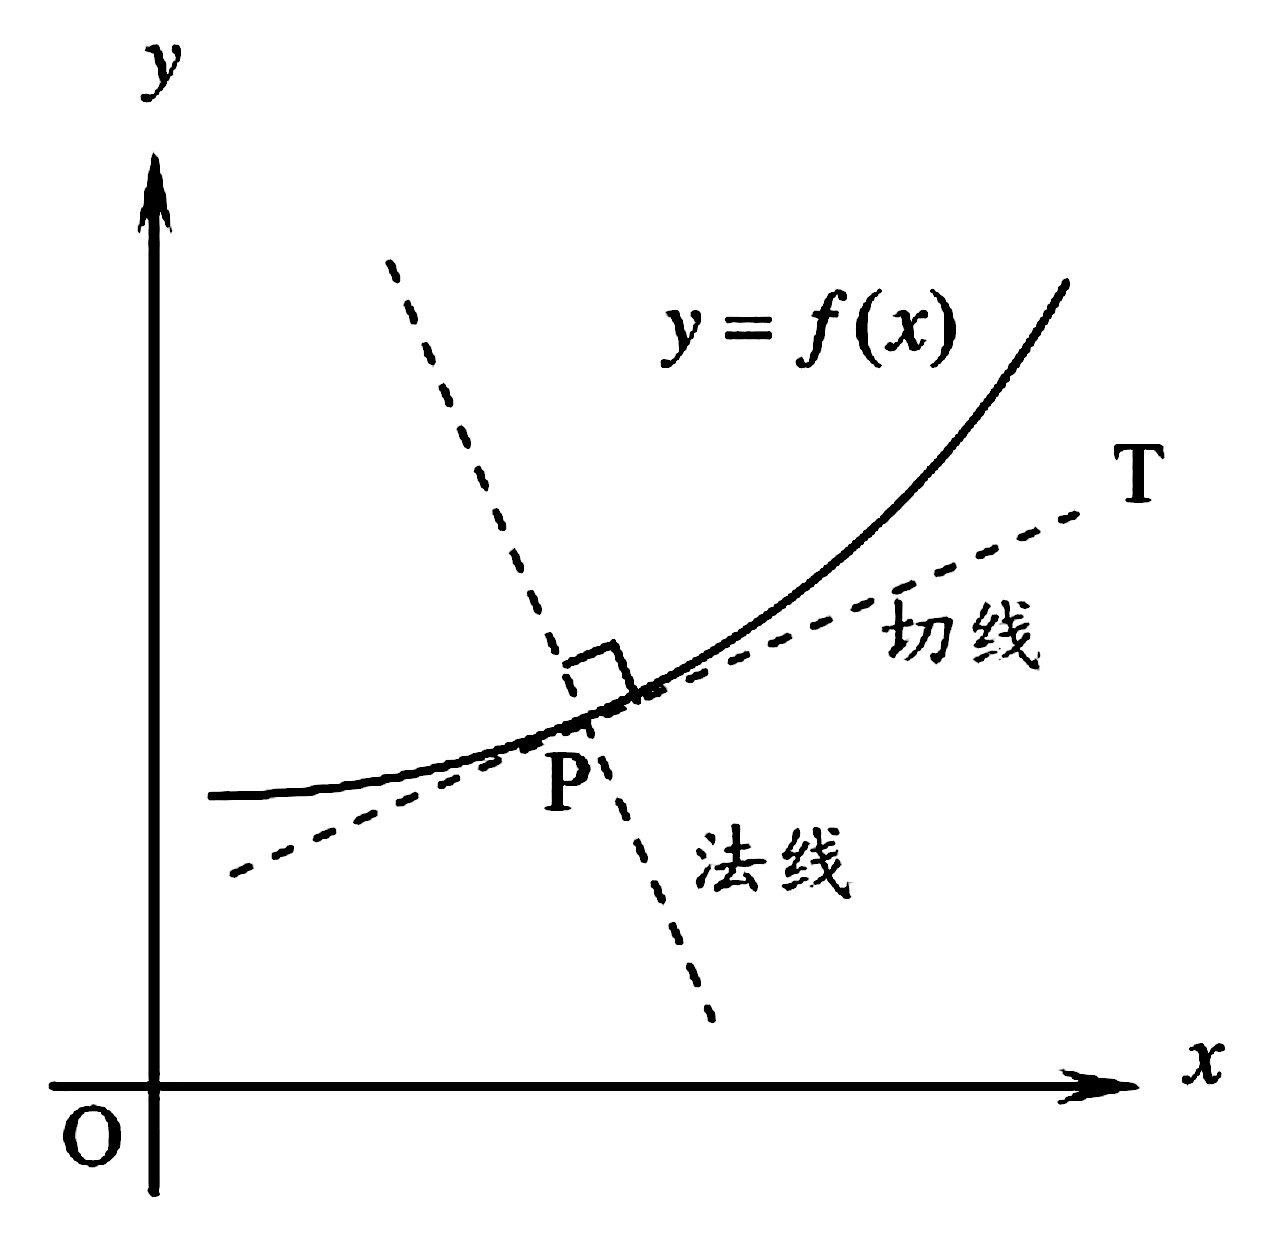
\includegraphics[scale=0.25]{assets/26-1.png}
    \end{center}
\end{multicols}

\subsection{Practice 1}
\begin{enumerate}
      \item Find the equations of tangent and normal to the curve $y = x^3$ where $x = 2$.
            \sol{} \vspace{-1cm}
            \begin{multicols}{2}
                  \begin{flalign*}
                        y              & = x^3  & \\
                        \dfrac{dy}{dx} & = 3x^2
                  \end{flalign*}
                  At $x = 2$, $y = (2)^3 = 8$
                  \begin{flalign*}
                        \text{Gradient of tangent } \dfrac{dy}{dx} & = 3(2)^2 = 12    & \\
                        \text{Gradient of normal }                 & = -\dfrac{1}{12}
                  \end{flalign*}
                  \vfill\null
                  \begin{flalign*}
                        \therefore\ \text{Equation of tangent is } y - 8 & = 12(x - 2)             & \\
                        y                                                & = 12x - 16              & \\
                        \text{Equation of normal is } y - 8              & = -\dfrac{1}{12}(x - 2) & \\
                        12y - 96                                         & = -x + 2                & \\
                        x + 12y                                          & = 98                    & \\
                  \end{flalign*}
                  \vfill\null
            \end{multicols}
            \vspace{-1cm}

      \item Given that the gradient of tangent to the curve $y = x^2 - 2x + 3$ at point $Q$
            is $4$, find the coordinates of the point $Q$. \sol{}
            \begin{flalign*}
                  y              & = x^2 - 2x + 3 & \\
                  \dfrac{dy}{dx} & = 2x - 2
            \end{flalign*}
            At point $Q$, $\dfrac{dy}{dx} = 4$
            \begin{flalign*}
                  4 & = 2x - 2             & \\
                  x & = 3                  & \\
                  y & = 3^2 - 2(3) + 3 = 6
            \end{flalign*}
            $\therefore$ Coordinates of point $Q$ is $(3, 6)$.
            \vfill\null

      \item Find the equations of the tangent and normal to the curve $x^3 - 2xy + y^2 = 1$
            at point $(1, 2)$. \sol{}
            \begin{flalign*}
                  x^3 - 2xy + y^2                                 & = 1                          & \\
                  3x^2 - 2y - 2x\dfrac{dy}{dx} + 2y\dfrac{dy}{dx} & = 0                          & \\
                  (2x - 2y) \dfrac{dy}{dx}                        & = 3x^2 - 2y                  & \\
                  \dfrac{dy}{dx}                                  & = \dfrac{3x^2 - 2y}{2x - 2y}
            \end{flalign*}
            At point $(1, 2)$,
            \begin{flalign*}
                  \text{Gradient of tangent } \dfrac{dy}{dx} & = \dfrac{3(1)^2 - 2(2)}{2(1) - 2(2)} & \\
                                                             & = \dfrac{1}{2}                       & \\
                  \text{Gradient of normal }                 & = -2
            \end{flalign*}
            \begin{flalign*}
                  \therefore\ \text{Equation of tangent is } y - 2 & = \dfrac{1}{2}(x - 1) & \\
                  2y - 4                                           & = x - 1               & \\
                  x - 2y                                           & = -3                  & \\
                  \text{Equation of normal is } y - 2              & = -2(x - 1)           & \\
                  y - 2                                            & = -2x + 2             & \\
                  y                                                & = -2x + 4
            \end{flalign*}
            \vfill\null
\end{enumerate}
\newpage
\subsection{Exercise 26.1}
\begin{enumerate}
      \begin{multicols}{2}
            \item Find the equations of the tangent and normal to the curve $y = x^2 + 2$ at
            point $(2, 6)$. \sol{}
            \begin{flalign*}
                  y              & = x^2 + 2 & \\
                  \dfrac{dy}{dx} & = 2x
            \end{flalign*}
            At point $(2, 6)$,
            \begin{flalign*}
                  \text{Gradient of tangent } \dfrac{dy}{dx} & = 2(2) = 4      & \\
                  \text{Gradient of normal }                 & = -\dfrac{1}{4}
            \end{flalign*}
            \begin{flalign*}
                  \therefore\ \text{Equation of tangent is } y - 6 & = 4(x - 2)             & \\
                  y                                                & = 4x - 2               & \\
                  \text{Equation of normal is } y - 6              & = -\dfrac{1}{4}(x - 2) & \\
                  4y - 24                                          & = -x + 2               & \\
                  x + 4y                                           & = 26
            \end{flalign*}

            \item Find the equation of the tangent to the curve $y = 2x^3 - 3x^2 - 12x + 8$ where
            $x = 0$. \sol{}
            \begin{flalign*}
                  y              & = 2x^3 - 3x^2 - 12x + 8 & \\
                  \dfrac{dy}{dx} & = 6x^2 - 6x - 12
            \end{flalign*}
            At $x = 0$, $y = 8$
            \begin{flalign*}
                  \text{Gradient of tangent } \dfrac{dy}{dx}       & = 6(0)^2 - 6(0) - 12 = -12 & \\
                  \therefore\ \text{Equation of tangent is } y - 8 & = -12(x - 0)               & \\
                  y                                                & = -12x + 8
            \end{flalign*}
      \end{multicols}
      \vfill\null

      \begin{multicols}{2}
            \item Find the equation of the normal to the curve $y = 3x^3 - 4x + 7$ at point $(1,
                  6)$. \sol{}
            \begin{flalign*}
                  y              & = 3x^3 - 4x + 7 & \\
                  \dfrac{dy}{dx} & = 9x^2 - 4
            \end{flalign*}
            At point $(1, 6)$,
            \begin{flalign*}
                  \text{Gradient of tangent } \dfrac{dy}{dx} & = 9(1)^2 - 4 = 5 & \\
                  \text{Gradient of normal }                 & = -\dfrac{1}{5}
            \end{flalign*}
            \begin{flalign*}
                  \therefore\ \text{Equation of normal is } y - 6 & = -\dfrac{1}{5}(x - 1) & \\
                  5y - 30                                         & = -x + 1               & \\
                  x + 5y                                          & = 31
            \end{flalign*}

            \item Find the equation of the tangent to the curve $y = \dfrac{1}{1-x}$ where $x =
                  -1$. \sol{}
            \begin{flalign*}
                  y              & = \dfrac{1}{1-x}     & \\
                  \dfrac{dy}{dx} & = \dfrac{1}{(1-x)^2}
            \end{flalign*}
            At $x = -1$, $y = \dfrac{1}{2}$
            \begin{flalign*}
                  \text{Gradient of tangent } \dfrac{dy}{dx}                  & = \dfrac{1}{[1-(-1)]^2} = \dfrac{1}{4} & \\
                  \therefore\ \text{Equation of tangent is } y - \dfrac{1}{2} & = \dfrac{1}{4}(x + 1)                  & \\
                  4y - 2                                                      & = x+1                                  & \\
                  x - 4y + 3                                                  & = 0
            \end{flalign*}
      \end{multicols}
      \vfill\null

      \newpage
      \item Find the equations of the tangent and normal to the curve $y = 1 - 2x^2$ where
            $x = -2$. \sol{}
            \begin{flalign*}
                  y              & = 1 - 2x^2 & \\
                  \dfrac{dy}{dx} & = -4x
            \end{flalign*}
            At $x = -2$, $y = 1 - 2(-2)^2 = -7$
            \begin{flalign*}
                  \text{Gradient of tangent } \dfrac{dy}{dx} & = -4(-2) = 8    & \\
                  \text{Gradient of normal }                 & = -\dfrac{1}{8}
            \end{flalign*}
            \begin{flalign*}
                  \therefore\ \text{Equation of tangent is } y + 7 & = 8(x + 2)             & \\
                  y                                                & = 8x + 9               & \\
                  \text{Equation of normal is } y + 7              & = -\dfrac{1}{8}(x + 2) & \\
                  8y + 56                                          & = -x - 2               & \\
                  x + 8y + 58                                      & = 0
            \end{flalign*}

      \item Find the equation of the tangent to the curve $y = (x+1)(x-1)(x-3)$ where the
            curve intersects with the $x$-axis. \sol{}
            \begin{flalign*}
                  y              & = (x+1)(x-1)(x-3)    & \\
                                 & = (x^2 - 1)(x-3)     & \\
                                 & = x^3 - 3x^2 - x + 3 & \\
                  \dfrac{dy}{dx} & = 3x^2 - 6x - 1
            \end{flalign*}
            At $y = 0$, $x = -1, 1, 3$.

            When $x = -1$,
            \begin{flalign*}
                  \text{Gradient of tangent } \dfrac{dy}{dx}   & = 3(-1)^2 - 6(-1) - 1 = 8 & \\
                  \therefore\ \text{Equation of tangent is } y & = 8(x + 1)                & \\
                  y                                            & = 8x + 8
            \end{flalign*}
            When $x = 1$,
            \begin{flalign*}
                  \text{Gradient of tangent } \dfrac{dy}{dx}   & = 3(1)^2 - 6(1) - 1 = -4 & \\
                  \therefore\ \text{Equation of tangent is } y & = -4(x - 1)              & \\
                  y                                            & = -4x + 4
            \end{flalign*}
            When $x = 3$,
            \begin{flalign*}
                  \text{Gradient of tangent } \dfrac{dy}{dx}   & = 3(3)^2 - 6(3) - 1 = 8 & \\
                  \therefore\ \text{Equation of tangent is } y & = 8(x - 3)              & \\
                  y                                            & = 8x - 24
            \end{flalign*}

      \item Find the equation of the tangent to the curve $y = 4x^3 - 27x + 7$ that is
            parallel to the $x$-axis. \sol{}
            \begin{flalign*}
                  y              & = 4x^3 - 27x + 7 & \\
                  \dfrac{dy}{dx} & = 12x^2 - 27
            \end{flalign*}
            The tangent is parallel to the $x$-axis when $\dfrac{dy}{dx} = 0$.
            \begin{flalign*}
                  12x^2 - 27 & = 0               & \\
                  4x^2       & = 9               & \\
                  x          & = \pm\dfrac{3}{2}
            \end{flalign*}
            When $x = \dfrac{3}{2}$, $y = 4\left(\dfrac{3}{2}\right)^3 - 27\left(\dfrac{3}{2}\right) + 7 = -20$
            \begin{flalign*}
                  \therefore\ \text{Equation of tangent is } y + 20 & = 0(x - \dfrac{3}{2}) & \\
                  y                                                 & = -20
            \end{flalign*}

            When $x = -\dfrac{3}{2}$, $y = 4\left(-\dfrac{3}{2}\right)^3 -
                  27\left(-\dfrac{3}{2}\right) + 7 = 34$
            \begin{flalign*}
                  \therefore\ \text{Equation of tangent is } y - 34 & = 0(x + \dfrac{3}{2}) & \\
                  y                                                 & = 34
            \end{flalign*}

      \item Find the equation of the tangent to the curve $y = 11x - 3x^2$ that is parallel
            to the line $x + y - 2 = 0$. \sol{}
            \begin{flalign*}
                  x + y - 2 & = 0      & \\
                  y         & = -x + 2
            \end{flalign*}
            The gradient of the line $x + y - 2 = 0$ is $-1$.
            \begin{flalign*}
                  y              & = 11x - 3x^2 & \\
                  \dfrac{dy}{dx} & = 11 - 6x
            \end{flalign*}
            The tangent is parallel to the line $x + y - 2 = 0$ when $\dfrac{dy}{dx} = -1$.
            \begin{flalign*}
                  11 - 6x & = -1 & \\
                  6x      & = 12 & \\
                  x       & = 2
            \end{flalign*}
            When $x = 2$, $y = 11(2) - 3(2)^2 = 10$
            \begin{flalign*}
                  \therefore\ \text{Equation of tangent is } y - 10 & = -1(x - 2) & \\
                  y                                                 & = -x + 12
            \end{flalign*}
            \begin{multicols}{2}
                  \item Find the equations of the tangent and normal to the curve $y = \ln{(2x - 1)}$
                  where $x=1$. \sol{}
                  \begin{flalign*}
                        y              & = \ln{(2x - 1)}     & \\
                        \dfrac{dy}{dx} & = \dfrac{2}{2x - 1}
                  \end{flalign*}
                  At $x = 1$, $y = \ln{(2(1) - 1)} = \ln{1} = 0$
                  \begin{flalign*}
                        \text{Gradient of tangent } \dfrac{dy}{dx} & = \dfrac{2}{2(1) - 1} = 2 & \\
                        \text{Gradient of normal }                 & = -\dfrac{1}{2}
                  \end{flalign*}
                  \begin{flalign*}
                        \therefore\ \text{Equation of tangent is } y - 0 & = 2(x - 1)             & \\
                        y                                                & = 2x - 2               & \\
                        \text{Equation of normal is } y - 0              & = -\dfrac{1}{2}(x - 1) & \\
                        2y                                               & = -x + 1               & \\
                        x + 2y                                           & = 1
                  \end{flalign*}
                  \item If the straight line $y = 8x + k$ is the tangent to the curve $y = x^2 + 4x -
                        3$, find the value of $k$. \sol{}

                  The gradient of the tangent line is $8$.
                  \begin{flalign*}
                        y              & = x^2 + 4x - 3 & \\
                        \dfrac{dy}{dx} & = 2x + 4       & \\
                        8              & = 2x + 4       & \\
                        x              & = 2
                  \end{flalign*}
                  When $x = 2$, $y = 2^2 + 4(2) - 3 = 9$

                  Substituting $x = 2$ and $y = 9$ into $y = 8x + k$,
                  \begin{flalign*}
                        9 & = 8(2) + k & \\
                        k & = -7
                  \end{flalign*}
            \end{multicols}

            \begin{multicols}{2}
                  \item Given that the gradient of tangent to the curve $y = ax + bx^2$ at point $(1,
                        0)$ is $\dfrac{1}{2}$, find the value of $a$ and $b$. \sol{}
                  \begin{flalign*}
                        y              & = ax + bx^2 & \\
                        \dfrac{dy}{dx} & = a + 2bx
                  \end{flalign*}
                  At point $(1, 0)$,
                  \begin{flalign*}
                        a(1) + b(1)^2                              & = 0                         & \\
                        a + b                                      & = 0\ \cdots\ (1)            & \\
                        \text{Gradient of tangent } \dfrac{dy}{dx} & = a + 2b(1) = \dfrac{1}{2}  & \\
                        a + 2b                                     & = \dfrac{1}{2}\ \cdots\ (2)
                  \end{flalign*}
                  Solving $(1)$ and $(2)$, $b = \dfrac{1}{2}$ and $a = -\dfrac{1}{2}$.
                  \vfill\null

                  \item If $x + y + 2 = 0$ is the equation of tangent to the curve $y = ax^2 + bx$
                  where $x = 1$, find the value of $a$ and $b$. \sol{}
                  \begin{flalign*}
                        x + y + 2 & = 0      & \\
                        y         & = -x - 2
                  \end{flalign*}
                  The gradient of the tangent line is $-1$.
                  \begin{flalign*}
                        y              & = ax^2 + bx & \\
                        \dfrac{dy}{dx} & = 2ax + b
                  \end{flalign*}
                  At $x = 1$, $y = -1 - 2 = -3$
                  \begin{flalign*}
                        -3                                         & = a(1)^2 + b(1)   & \\
                        a + b                                      & = -3\ \cdots\ (1) & \\
                        \text{Gradient of tangent } \dfrac{dy}{dx} & = 2a(1) + b = -1  & \\
                        2a + b                                     & = -1\ \cdots\ (2)
                  \end{flalign*}
                  Solving $(1)$ and $(2)$, $a = 2$ and $b = -5$.
            \end{multicols}

            \newpage
            \begin{multicols}{2}
                  \item Given that the gradient of tangent to the curve $y = x^3 - 6x^2 + 10x - 5$ at
                  point $P$ is $-2$, find the coordinates of $P$. \sol{}
                  \begin{flalign*}
                        y              & = x^3 - 6x^2 + 10x - 5 & \\
                        \dfrac{dy}{dx} & = 3x^2 - 12x + 10
                  \end{flalign*}
                  At point $P$, $\dfrac{dy}{dx} = -2$
                  \begin{flalign*}
                        -2              & = 3x^2 - 12x + 10 & \\
                        3x^2 - 12x + 12 & = 0               & \\
                        x^2 - 4x + 4    & = 0               & \\
                        (x - 2)^2       & = 0               & \\
                        x               & = 2
                  \end{flalign*}
                  When $x = 2$, $y = 2^3 - 6(2)^2 + 10(2) - 5 = -1$

                  $\therefore$ Coordinates of point $P$ is $(2, -1)$.
                  \vfill\null

                  \item Prove that the tangent lines to the curve $y = x^2 - 3x + 1$ and the curve
                  $x(y+3) = 4$ at point $(2, -1)$ are perpendicular to each other. \prooff{}
                  \begin{flalign*}
                        y              & = x^2 - 3x + 1 & \\
                        \dfrac{dy}{dx} & = 2x - 3
                  \end{flalign*}
                  At point $(2, -1)$,
                  \begin{flalign*}
                        \text{Gradient of tangent } \dfrac{dy}{dx} & = 2(2) - 3 = 1
                  \end{flalign*}
                  \begin{flalign*}
                        x(y+3)         & = 4                & \\
                        y              & = \dfrac{4}{x} - 3 & \\
                        \dfrac{dy}{dx} & = -\dfrac{4}{x^2}
                  \end{flalign*}
                  At point $(2, -1)$,
                  \begin{flalign*}
                        \text{Gradient of tangent } \dfrac{dy}{dx} & = -\dfrac{4}{(2)^2} = -1
                  \end{flalign*}
                  Since the product of the gradients of the two lines is $1 \times -1 = -1$, the two lines are perpendicular to each other. \qed
            \end{multicols}

            \begin{multicols}{2}
                  \item Find the equations of the tangent and normal to the curve $x^2 - xy + y^2 = 7$
                  at point $(-2, -3)$. \sol{}
                  \begin{flalign*}
                        x^2 - xy + y^2                              & = 7                      & \\
                        2x - y - x\dfrac{dy}{dx} + 2y\dfrac{dy}{dx} & = 0                      & \\
                        (2y - x) \dfrac{dy}{dx}                     & = y - 2x                 & \\
                        \dfrac{dy}{dx}                              & = \dfrac{y - 2x}{2y - x}
                  \end{flalign*}
                  At point $(-2, -3)$,
                  \begin{flalign*}
                        \text{Gradient of tangent } \dfrac{dy}{dx} & = \dfrac{-3 - 2(-2)}{2(-3) - (-2)} = -\dfrac{1}{4} & \\
                        \text{Gradient of normal }                 & = 4
                  \end{flalign*}
                  \vspace{-1cm}
                  \begin{flalign*}
                        \therefore\ \text{Equation of tangent is } y + 3 & = -\dfrac{1}{4}(x + 2) & \\
                        4y + 12                                          & = -x - 2               & \\
                        x + 4y + 14                                      & = 0                    & \\
                        \text{Equation of normal is } y + 3              & = 4(x + 2)             & \\
                        y                                                & = 4x + 5
                  \end{flalign*}

                  \item Find the equation of tangent to the curve $y^2 + y = 2\sin x$ at point $(0,
                        -1)$.
                  \begin{flalign*}
                        y^2 + y = 2\sin x                           & \\
                        2y\dfrac{dy}{dx} + \dfrac{dy}{dx} = 2\cos x & \\
                        (2y + 1) \dfrac{dy}{dx} = 2\cos x           & \\
                        \dfrac{dy}{dx} = \dfrac{2\cos x}{2y + 1}
                  \end{flalign*}
                  At point $(0, -1)$,
                  \begin{flalign*}
                        \text{Gradient of tangent } \dfrac{dy}{dx}       & = \dfrac{2\cos 0}{2(-1) + 1} = -2 & \\
                        \therefore\ \text{Equation of tangent is } y + 1 & = -2(x - 0)                       & \\
                        y                                                & = -2x - 1
                  \end{flalign*}
            \end{multicols}
\end{enumerate}

\newpage

\section{Increasing and Decreasing Functions}

\subsection*{Monotonic Functions}

For a function $f(x)$ being defined in the interval $D$,
\begin{enumerate}
    \item For any two numbers $x_1$ and $x_2$ in $D$, when $x_1 < x_2$, $f(x)$ is an
          increasing function in the interval $D$, as shown in the figure below.
          \begin{center}
              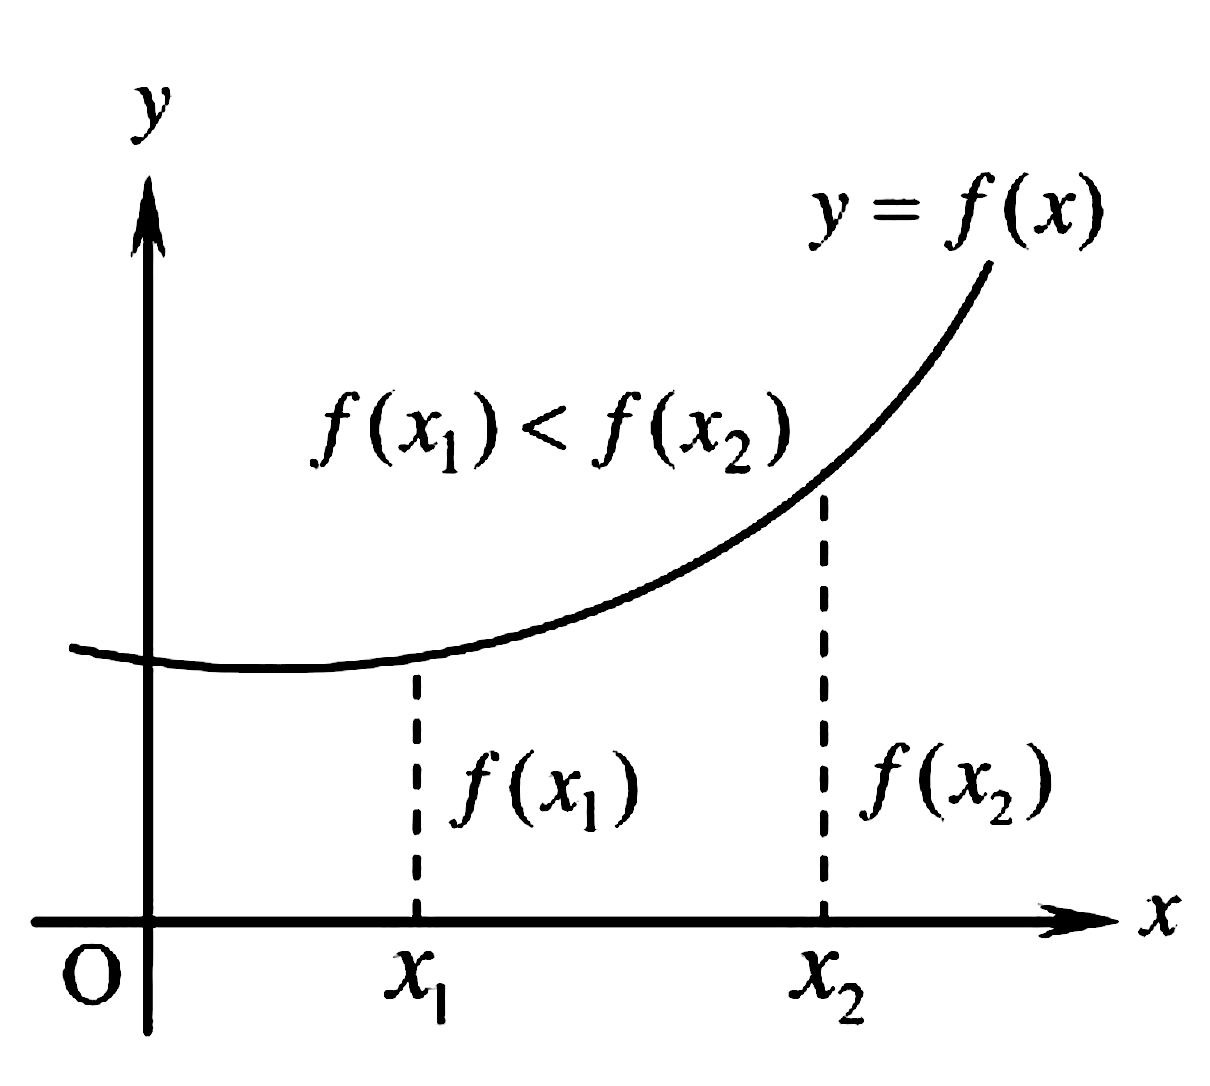
\includegraphics[scale=0.25]{assets/26-2.png}
          \end{center}
    \item For any two numbers $x_1$ and $x_2$ in $D$, when $x_1 > x_2$, $f(x)$ is a
          decreasing function in the interval $D$, as shown in the figure below.
          \begin{center}
              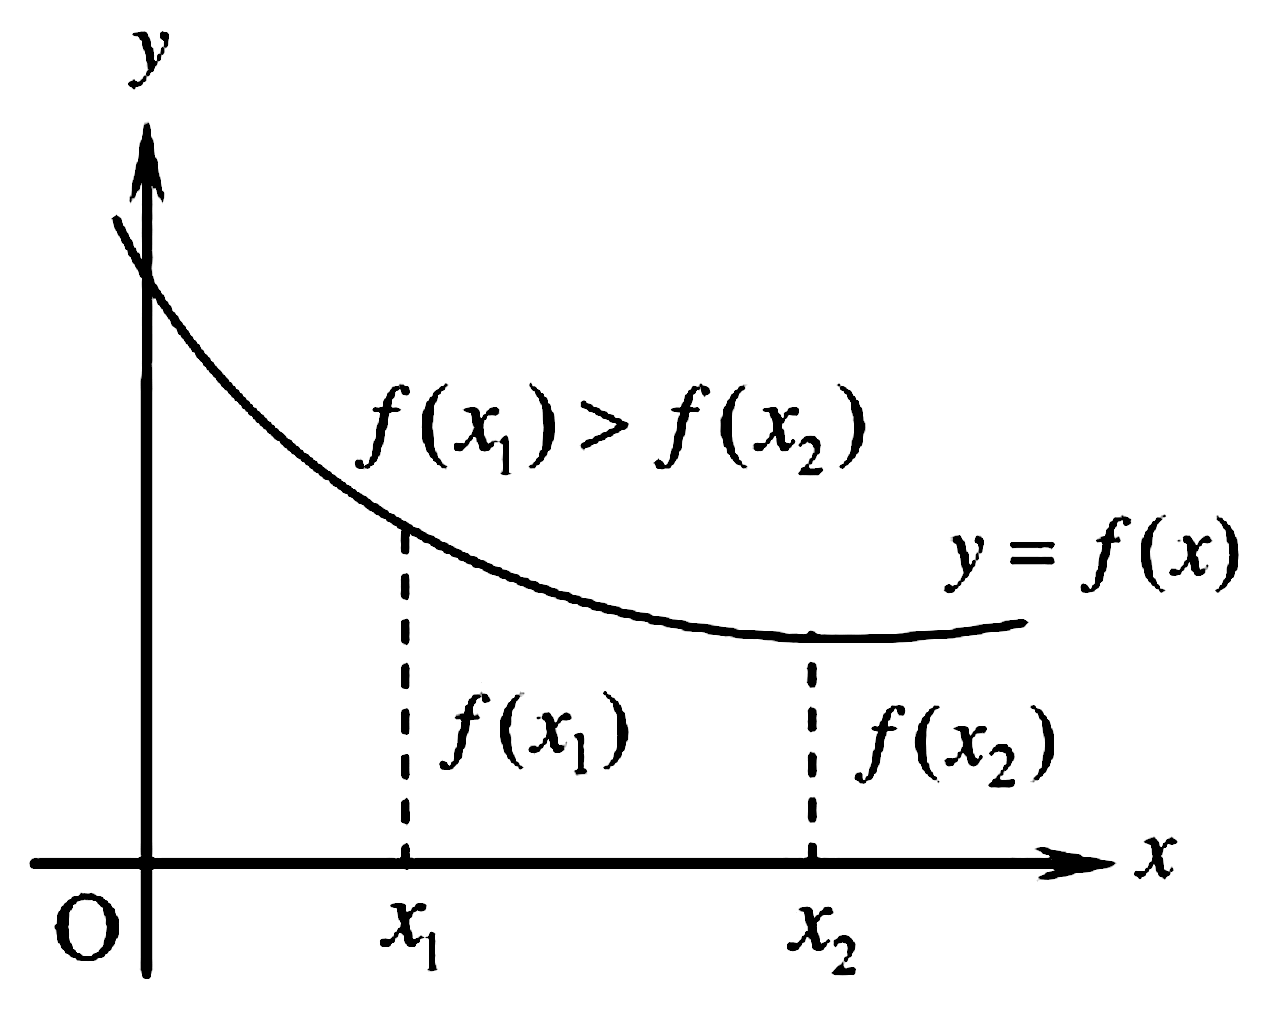
\includegraphics[scale=0.25]{assets/26-3.png}
          \end{center}
\end{enumerate}
If $f(x)$ is an increasing function or a decreasing function in the interval $D$, we call $f(x)$ a monotonic function in the interval $D$.
\begin{center}
    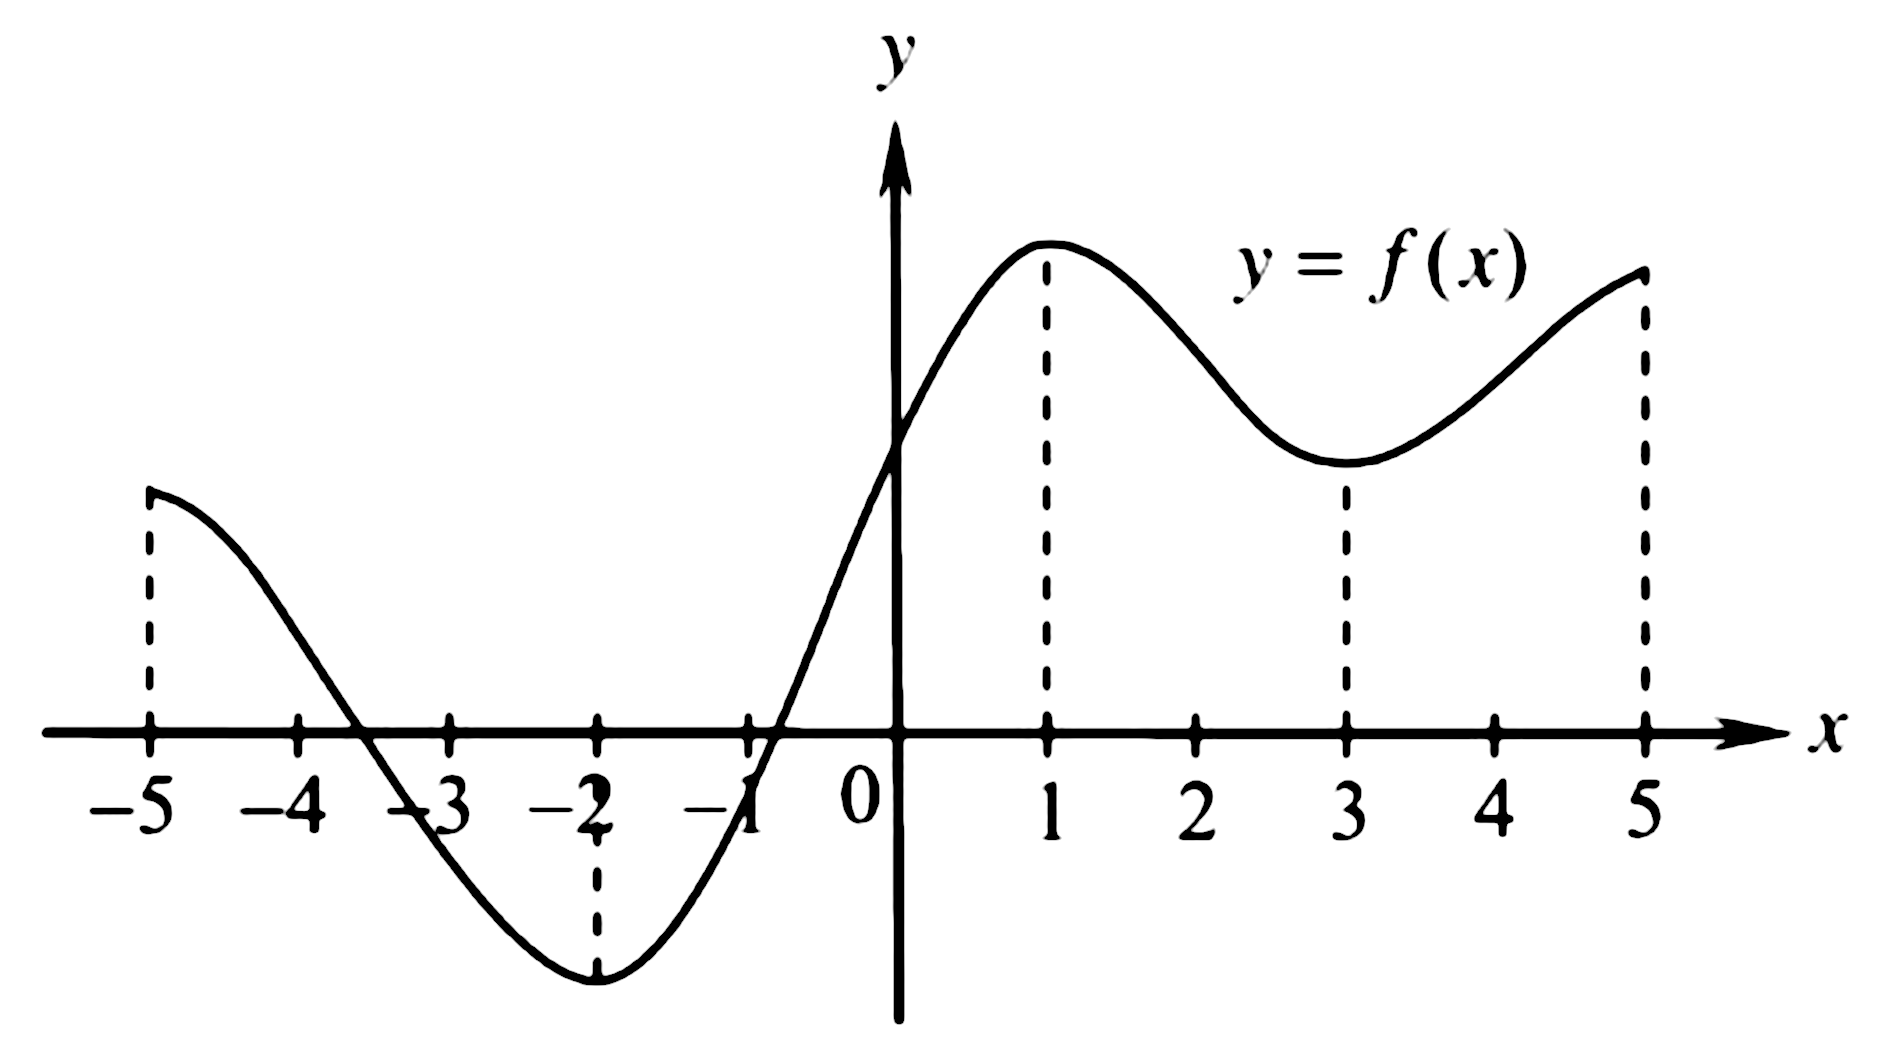
\includegraphics[scale=0.25]{assets/26-4.png}
\end{center}
The curve shown in the diagram above is the graph of the function $f(x)$ in the
interval $[-5, 5]$. From the graph, we can see that the function $f(x)$ is a
decreasing function in the intervals $[-5, 2]$ and $[1, 3]$, and an increasing
function in the interval $[-2, 1]$ and $[3, 5]$.
\newpage

\subsection*{How to Judge the Increase or Decrease of Functions}

As shown in the diagram below, when the function $f(x)$ is an increasing
function in the interval $[a, b]$, the gradient of the tangent to the curve at
any point in the interval $(a, b)$ is positive, i.e. $f'(x) > 0$; when the
function $f(x)$ is a decreasing function in the interval $[b, c]$, the gradient
of the tangent to the curve at any point in the interval $(b, c)$ is negative,
i.e. $f'(x) < 0$.
\begin{center}
    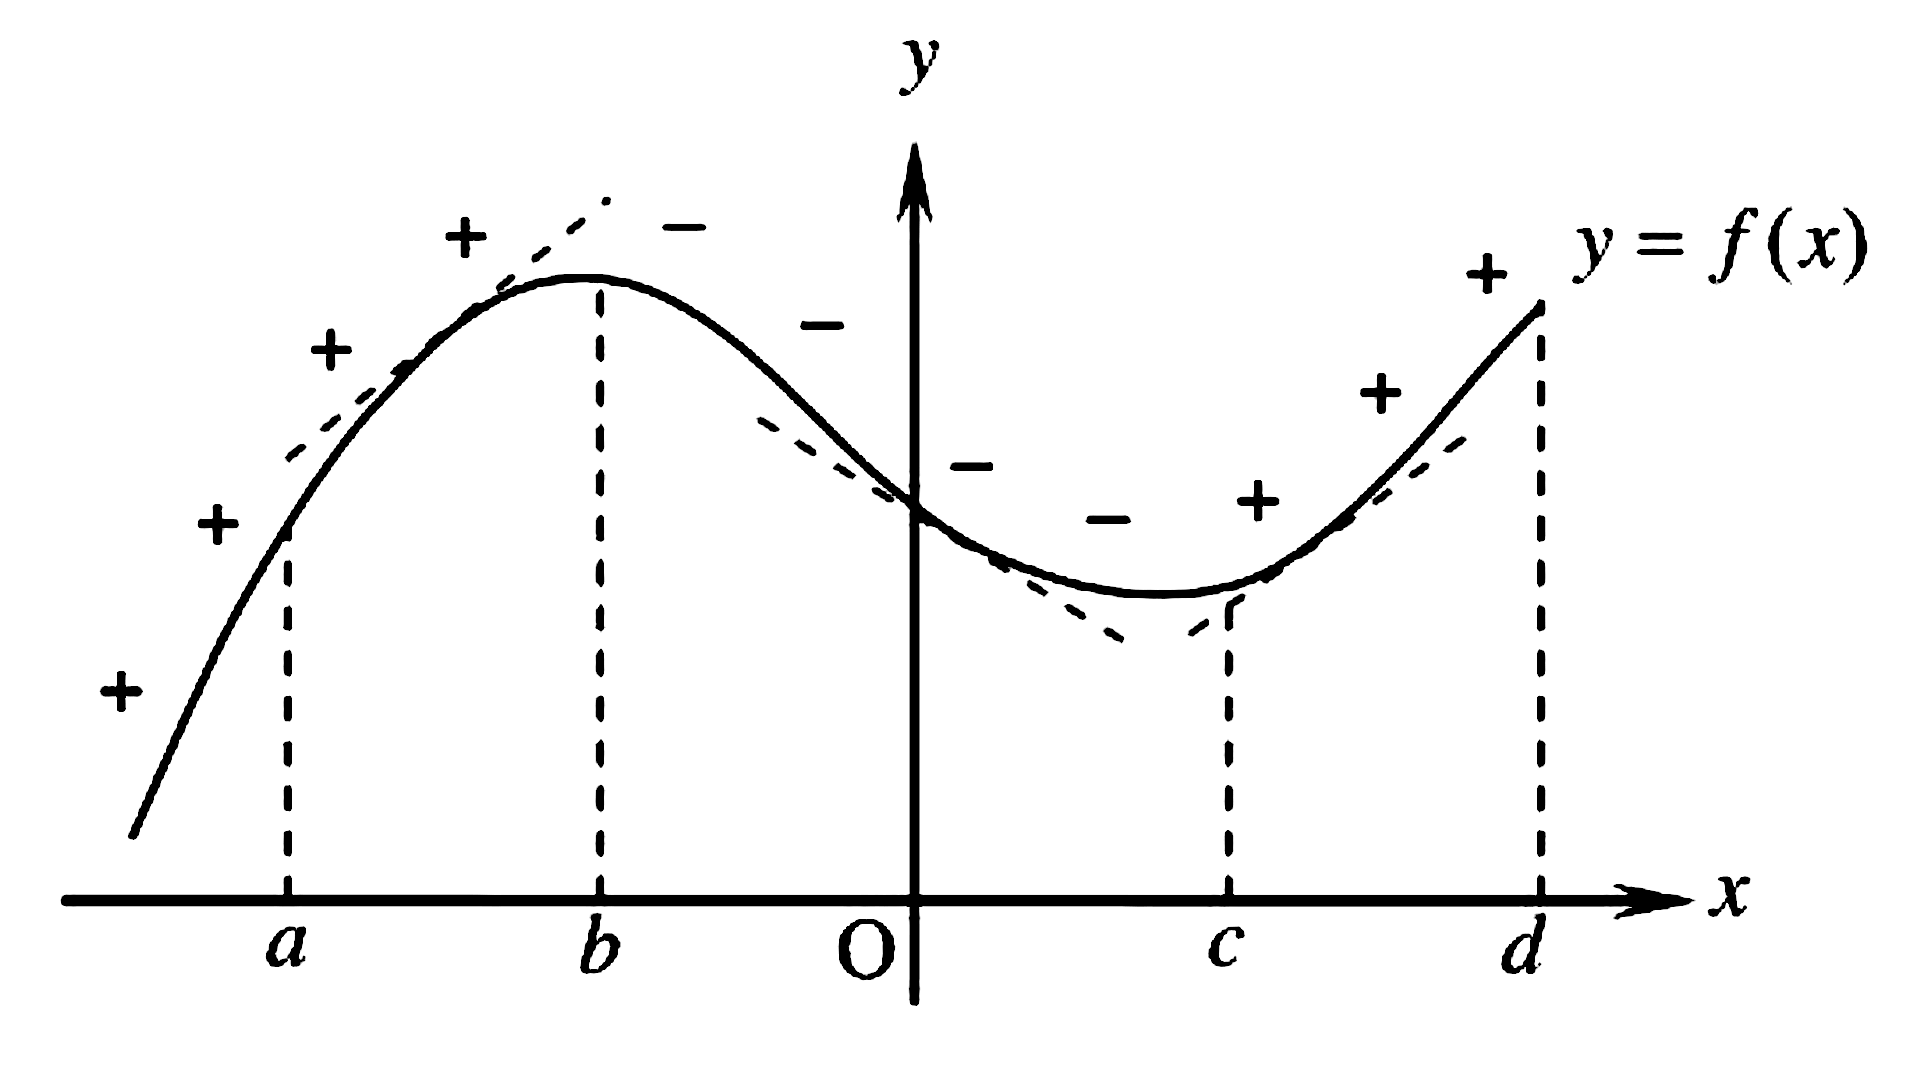
\includegraphics[scale=0.25]{assets/26-5.png}
\end{center}
Therefore, we can judge whether a function is an increasing function or a decreasing function in an interval by the sign of the derivative value of the function in the interval:
\begin{center}
    \framebox{
        \parbox[t][3.8cm]{14cm}{ \addvspace{0.6cm} \hspace{0.4cm}Let $f(x)$ be a continuous
            function defined in the interval $[a, b]$, and can be differentiated in

            \hspace{0.4cm}the interval $(a, b)$.

            \begin{itemize}[leftmargin=0.76cm]
                \item In the interval $(a, b)$, if $f'(x) > 0$, then $f(x)$ is an increasing function
                      in the interval $[a, b]$.
                \item In the interval $(a, b)$, if $f'(x) < 0$, then $f(x)$ is a decreasing function
                      in the interval $[a, b]$.
            \end{itemize} }}
\end{center}
\vspace{0.9em}

\subsection{Practice 2}

\begin{enumerate}
    \begin{multicols}{2}
        \item $\displaystyle\int_2^8 x d x$
        \sol{}
        \begin{flalign*}
            I & = \left[\dfrac{1}{2}x^2\right]_2^8 & \\
              & = \dfrac{1}{2}(64 - 4)             & \\
              & = 30
        \end{flalign*}

        \item $\displaystyle\int_{-2}^4 x^3 d x$
        \sol{}
        \begin{flalign*}
            I & = \left[\dfrac{1}{4}x^4\right]_{-2}^4 & \\
              & = \dfrac{1}{4}(256 - 16)              & \\
              & = 60
        \end{flalign*}
    \end{multicols}
    \begin{multicols}{2}
        \item $\displaystyle\int_{-\pi}^\pi \cos x d x$
        \sol{}
        \begin{flalign*}
            I & = \bigg[\sin x\bigg]_{-\pi}^\pi & \\
              & = \sin\pi - \sin(-\pi)          & \\
              & = 0 - 0                         & \\
              & = 0
        \end{flalign*}

        \item $\displaystyle\int_0^{\frac{\pi}{4}} \sec ^2 x d x$
        \sol{}
        \begin{flalign*}
            I & = \bigg[\tan x\bigg]_0^{\frac{\pi}{4}} & \\
              & = \tan\dfrac{\pi}{4} - \tan 0          & \\
              & = 1 - 0                                & \\
              & = 1
        \end{flalign*}
    \end{multicols}
\end{enumerate}
\subsection{Exercise 26.2}

\noindent \hspace{1.2em}\textit{Determine which intervals the following functions is an increasing function or a decreasing function.}
\begin{enumerate}
    \begin{multicols}{2}
        \item $f(x)=x^2-2 x+4$
        \sol{}
        \begin{flalign*}
            f'(x)  & = 2x - 2 & \\
            2x - 2 & = 0      & \\
            x      & = 1
        \end{flalign*}
        In the interval $(-\infty,1)$, $f'(x)<0$, so $f(x)$ is a decreasing function in the interval $(-\infty,1]$.

        In the interval $(1,\infty)$, $f'(x)>0$, so $f(x)$ is an increasing function in
        the interval $[1,\infty)$. \vfill\null

                        \item $f(x)=2 x^3-6 x^2+7$
                        \sol{}
                        \begin{flalign*}
                            f'(x)      & = 6x^2 - 12x          & \\
                            6x^2 - 12x & = 0                   & \\
                            x(x - 2)   & = 0                   & \\
                            x          & = 0 \text{ or } x = 2
                        \end{flalign*}
                        In the interval $(-\infty,0)$, $f'(x)>0$, so $f(x)$ is an increasing function in the interval $(-\infty,0]$.

        In the interval $(0,2)$, $f'(x)<0$, so $f(x)$ is a decreasing function in the
        interval $[0,2]$.

        In the interval $(2,\infty)$, $f'(x)>0$, so $f(x)$ is an increasing function in
        the interval $[2,\infty)$.
    \end{multicols}
    \vfill\null

    \begin{multicols}{2}
        \item $f(x)=x^3+x$
        \sol{}
        \begin{flalign*}
            f'(x)    & = 3x^2 + 1        & \\
            3x^2 + 1 & = 0               & \\
            x^2      & = -\frac{1}{3}      \\
            x        & \notin \mathbb{R}
        \end{flalign*}
        Since $f'(x)>0$ for all $x \in \mathbb{R}$, $f(x)$ is an increasing function.
        \vfill\null

        \item $f(x)=2+3 x-x^3$
        \sol{}
        \begin{flalign*}
            f'(x)    & = 3 - 3x^2 & \\
            3 - 3x^2 & = 0        & \\
            x^2      & = 1          \\
            x        & = \pm 1
        \end{flalign*}
        In the interval $(-\infty,-1)$, $f'(x)<0$, so $f(x)$ is a decreasing function in the interval $(-\infty,-1]$.

        In the interval $(-1,1)$, $f'(x)>0$, so $f(x)$ is an increasing function in the
        interval $[-1,1]$.

        In the interval $(1,\infty)$, $f'(x)<0$, so $f(x)$ is a decreasing function in
        the interval $[1,\infty)$.
    \end{multicols}
    \vfill\null
    \newpage

    \begin{multicols}{2}
        \item $f(x)=x^2(x-3)$
        \sol{}
        \begin{flalign*}
            f(x)      & = x^3 - 3x^2          & \\
            f'(x)     & = 3x^2 - 6x           & \\
            3x^2 - 6x & = 0                   & \\
            x(x - 2)  & = 0                   & \\
            x         & = 0 \text{ or } x = 2
        \end{flalign*}
        In the interval $(-\infty,0)$, $f'(x)>0$, so $f(x)$ is an increasing function in the interval $(-\infty,0]$.

        In the interval $(0,2)$, $f'(x)<0$, so $f(x)$ is a decreasing function in the
        interval $[0,2]$.

        In the interval $(2,\infty)$, $f'(x)>0$, so $f(x)$ is an increasing function in
        the interval $[2,\infty)$. \vfil\null

                        \item $f(x)=3 x^4+2 x^3-3 x^2-2$
                        \sol{}
                        \begin{flalign*}
                            f'(x)                    & = 12x^3 + 6x^2 - 6x         & \\
                            12x^3 + 6x^2             & = 6x                        & \\
                            x(2x^2 + x - 1)          & = 0                         & \\
                            x(x + 1)(2x - 1)         & = 0                         & \\
                            x = 0 \text{ or } x = -1 & \text{ or } x = \frac{1}{2}
                        \end{flalign*}
                        In the interval $(-\infty,-1)$, $f'(x)<0$, so $f(x)$ is a decreasing function in the interval $(-\infty,-1]$.

        In the interval $(-1,0)$, $f'(x)>0$, so $f(x)$ is an increasing function in the
        interval $[-1,0]$.

        In the interval $(0,\frac{1}{2})$, $f'(x)<0$, so $f(x)$ is a decreasing
        function in the interval $[0,\frac{1}{2}]$.

        In the interval $(\frac{1}{2},\infty)$, $f'(x)>0$, so $f(x)$ is an increasing
        function in the interval $[\frac{1}{2},\infty)$.
    \end{multicols}
    \vfill\null

    \begin{multicols}{2}
        \item $f(x)=\dfrac{x}{x^2+1}$
        \sol{}
        \begin{flalign*}
            f'(x)   & = \frac{(x^2+1) - x(2x)}{(x^2+1)^2} & \\
                    & = \frac{1 - x^2}{(x^2+1)^2}         & \\
            1 - x^2 & = 0                                 & \\
            x^2     & = 1                                 & \\
            x       & = \pm 1
        \end{flalign*}
        In the interval $(-\infty,-1)$, $f'(x) < 0$, so $f(x)$ is a decreasing function in the interval $(-\infty,-1]$.

        In the interval $(-1,1)$, $f'(x) > 0$, so $f(x)$ is an increasing function in
        the interval $[-1,1]$.

        In the interval $(1,\infty)$, $f'(x) < 0$, so $f(x)$ is a decreasing function
        in the interval $[1,\infty)$.\columnbreak

        \item $f(x)=\cos 2 x, 0 \leq x \leq \pi$
        \sol{}
        \begin{flalign*}
            f'(x)      & = -2 \sin 2x                       & \\
            -2 \sin 2x & = 0                                & \\
            \sin 2x    & = 0                                & \\
            2x         & = \sin^{-1} 0                      & \\
            x          & = 0 \text{ or } x = \dfrac{\pi}{2}
        \end{flalign*}
        In the interval $\left[0,\dfrac{\pi}{2}\right]$, $f'(x) < 0$, so $f(x)$ is a decreasing function in the interval $\left[0,\dfrac{\pi}{2}\right]$.

        In the interval $\left[\dfrac{\pi}{2},\pi\right]$, $f'(x) > 0$, so $f(x)$ is an
        increasing function in the interval $\left[\dfrac{\pi}{2},\pi\right]$.
    \end{multicols}
    \vfill\null
\end{enumerate}

\section{Relative Maximum and Minimum Values of Functions}

As shown in the diagram below, the function value $f(a)$ at the point where
$x=a$ is the maximum compared to its nearby points, we call $f(a)$ the relative
maximum value; the function value $f(b)$ at the point where $x=b$ is the
minimum compared to its nearby points, we call $f(b)$ the relative minimum
value.
\begin{center}
    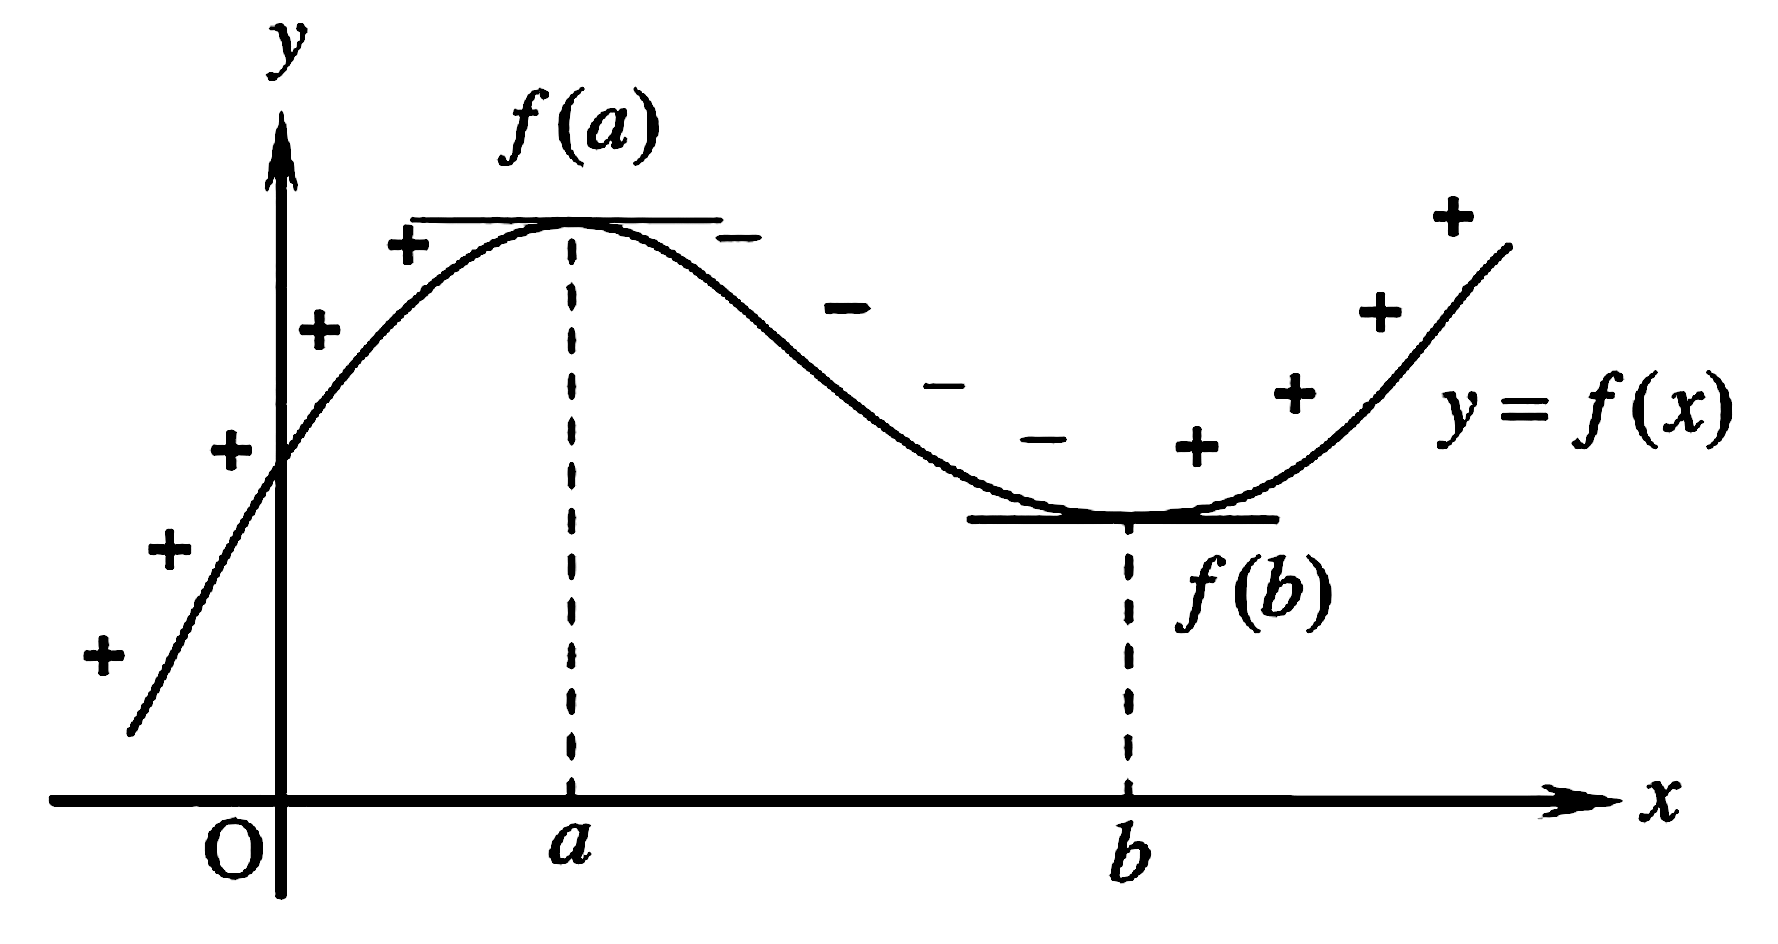
\includegraphics[scale=0.25]{assets/26-6.png}
\end{center}

\begin{center}
    \framebox{
        \parbox[t][5cm]{14cm}{ \addvspace{0.6cm} \hspace{0.4cm}Let $f(x)$ be a defined
            function near point $x=a$,
            \begin{itemize}
                \item \parbox[t]{12.5cm}{If the function value $f(a)$ is the maximum compared to its
                          nearby points, we say that $f(x)$ has a relative maximum value $f(a)$ at point
                          $x=a$, and the point $(a, f(a))$ is the relative maximum point of the
                          function;}
                \item \parbox[t]{12.5cm}{If the function value $f(a)$ is the minimum compared to its
                          nearby points, we say that $f(x)$ has a relative minimum value $f(a)$ at point
                          $x=a$, and the point $(a, f(a))$ is the relative minimum point of the
                          function.}
            \end{itemize}
        }}
\end{center}
\vspace{0.9em}

Relative maximum and minimum values are collectively known as the extreme
values, and the points where the extreme values occur are collectively known as
the extreme points.

From the diagram above, we can also see that the gradients of the tangent to
the curve at the extreme points are zero. Hence, the following theorem can be
obtained:
\begin{center}
    \framebox{
        \parbox[t][1.6cm]{14cm}{ \addvspace{0.4cm} \centering \parbox{13cm}{If the function $f(x)$ is differentiable at point $x=a$, and $f(x)$
                has a relative maximum or minimum value at point $x=a$, then $f'(a)=0$.} }}
\end{center}

\begin{multicols}{2}
    The points that satisfy $f'(x)=0$ are called the stationary points of the
    function.

    If the function can be differentiated at point $x=a$, then the extreme point
    must be a stationary point. However, the stationary point is not necessarily an
    extreme point. For example, the derivative of the function $f(x)=x^3$ is
    $f'(x)=3x^2$, and $f'(0)=0$, i.e. $O(0, 0)$ is a stationary point of the
    function $f(x)=x^3$, but it is not an extreme point of the function, as shown
    in the right diagram. \vfill{}\null{}

    \columnbreak
    \begin{center}
        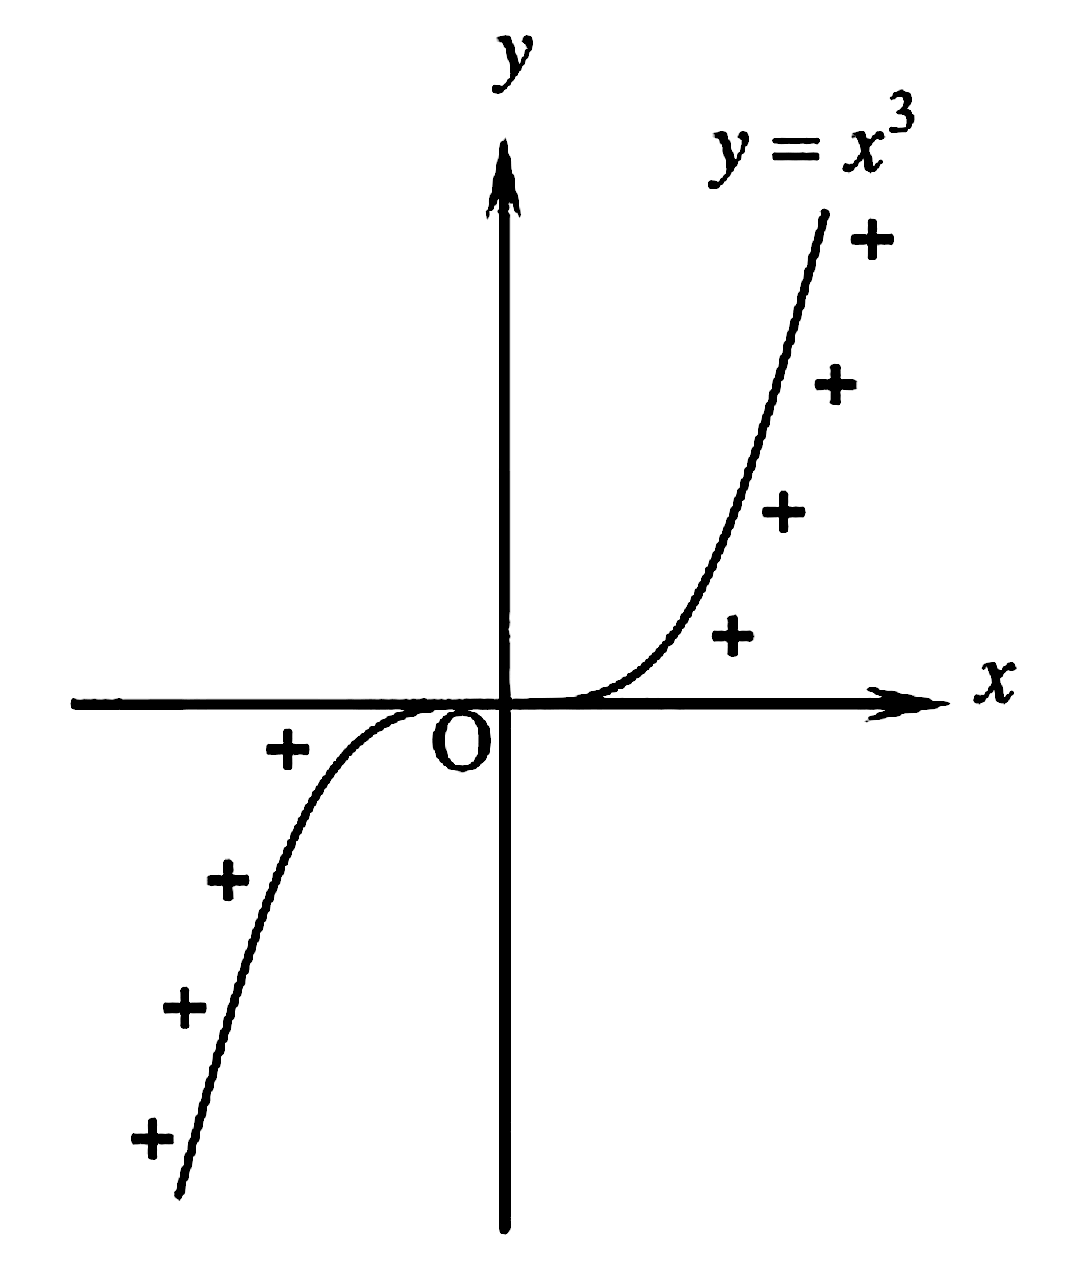
\includegraphics[scale=0.25]{assets/26-7.png}
    \end{center}
\end{multicols}

\subsection*{How to Find the Extreme Values of Functions}

\begin{enumerate}
    \item \textbf{First Derivative Test}

          The curve has a positive gradient of tangent to the left of the relative
          maximum point, and a negative gradient of tangent to the right; the curve has a
          negative gradient of tangent to the left of the relative minimum point, and a
          positive gradient of tangent to the right. Hence, the following theorem is
          obtained:
          \begin{center}
              \framebox{
                  \parbox[t][3.3cm]{14cm}{ \addvspace{0.4cm} \centering \parbox{13cm}{Let $f(x)$ be a function that is differentiable near point $x=a$, and
                          $f'(a) = 0$,
                          \begin{itemize}[leftmargin=0.4cm]
                              \item \parbox[t]{12.5cm}{If $f'(x) > 0$ to the left of $x=a$ and $f'(x) < 0$ to the right
                                        of $x=a$, then $f(a)$ is a relative maximum value;}
                              \item \parbox[t]{12.5cm}{If $f'(x) < 0$ to the left of $x=a$ and $f'(x) > 0$ to the right
                                        of $x=a$, then $f(a)$ is a relative minimum value.}
                          \end{itemize} }
                  }}
          \end{center}
          \vspace{0.9em}

    \item \textbf{Second Derivative Test}
          \begin{center}
              \framebox{
                  \parbox[t][2.5cm]{14cm}{ \addvspace{0.4cm} \centering \parbox{13cm}{Let $f(x)$ be a function that is second derivable near point $x=a$,
                          and $f'(a) = 0$,
                          \begin{itemize}[leftmargin=0.4cm]
                              \item \parbox[t]{12.5cm}{If $f''(a) < 0$, then $f(a)$ is a relative maximum value;}
                              \item \parbox[t]{12.5cm}{If $f''(a) > 0$, then $f(a)$ is a relative minimum value.}
                          \end{itemize} }
                  }}
          \end{center}

          Note that the second derivative test is invalid when $f''(a) = 0$, and the
          first derivative test should be used instead.
\end{enumerate}

\subsection{Practice 3}

\noindent \hspace{1.2em}\textit{
    Find the extreme values of the following functions (Question 1 to 4):
}

\begin{enumerate}
    \item $f(x)=x^2+x-6$
    \item $f(x)=2-x-x^2$
    \item $f(x)=\dfrac{1}{3} x^3-\dfrac{1}{2} x^2-2x+2$
    \item $f(x)=4 x-3 x^3$
\end{enumerate}

\noindent \hspace{1.2em}\textit{Find the coordinates of the extreme points of the following functions (Question 5 to 6):}
\begin{enumerate}[resume]
    \item $y=2 x^3-3 x^2-12 x-7$
    \item $y=x+\dfrac{1}{x}$
\end{enumerate}


\subsection{Exercise 26.3}

\noindent \hspace{1.2em}\textit{Find the extreme values of the following functions (Question 1 to 6):}
\begin{enumerate}
    \item $f(x)=\dfrac{1}{2} x^2-3 x$
    \item $f(x)=4+2 x-x^2$
    \item $f(x)=-2 x^2+4 x+7$
    \item $f(x)=3 x^2-2 x+1$
    \item $f(x)=2 x^3-9 x^2-24 x-12$
    \item $f(x)=15+9 x-3 x^2-x^3$
\end{enumerate}

\noindent \hspace{1.2em}\textit{Find the coordinates of the extreme points of the following functions (Question 7 to 11):}
\begin{enumerate}[resume]
    \item $f(x)=x\left(x^2-12\right)$
    \item $f(x)=4 x^3-3 x^2-6 x+2$
    \item $f(x)=x(x-8)(x-3)$
    \item $f(x)=4 x^2+\dfrac{1}{x}$
    \item $f(x)=x-2 \sin x, \quad-\pi<x<\pi$
    \item Find the stationery points of the function $f(x)=x^2(3-x)$, and determine
          whether the stationery points are relative maximum points or relative minimum
          points.
\end{enumerate}

\section{Absolute Maximum and Minimum Values of Functions}

Shown in the diagram below is the graph of the curve of the function $f(x)$ in
the interval $[a, b]$. From the diagram, we know that $f(x_1)$ and $f(x_3)$ are
the relative minimum value, while $f(x_2)$ is the relative maximum value. In
solving practical problems, we are often concerned with the maximum and minimum
values of the function in the entire domain. In the diagram below, the absolute
maximum value of the function $f(x)$ is $f(b)$, and the absolute minimum value
is $f(x_3)$.
\begin{center}
    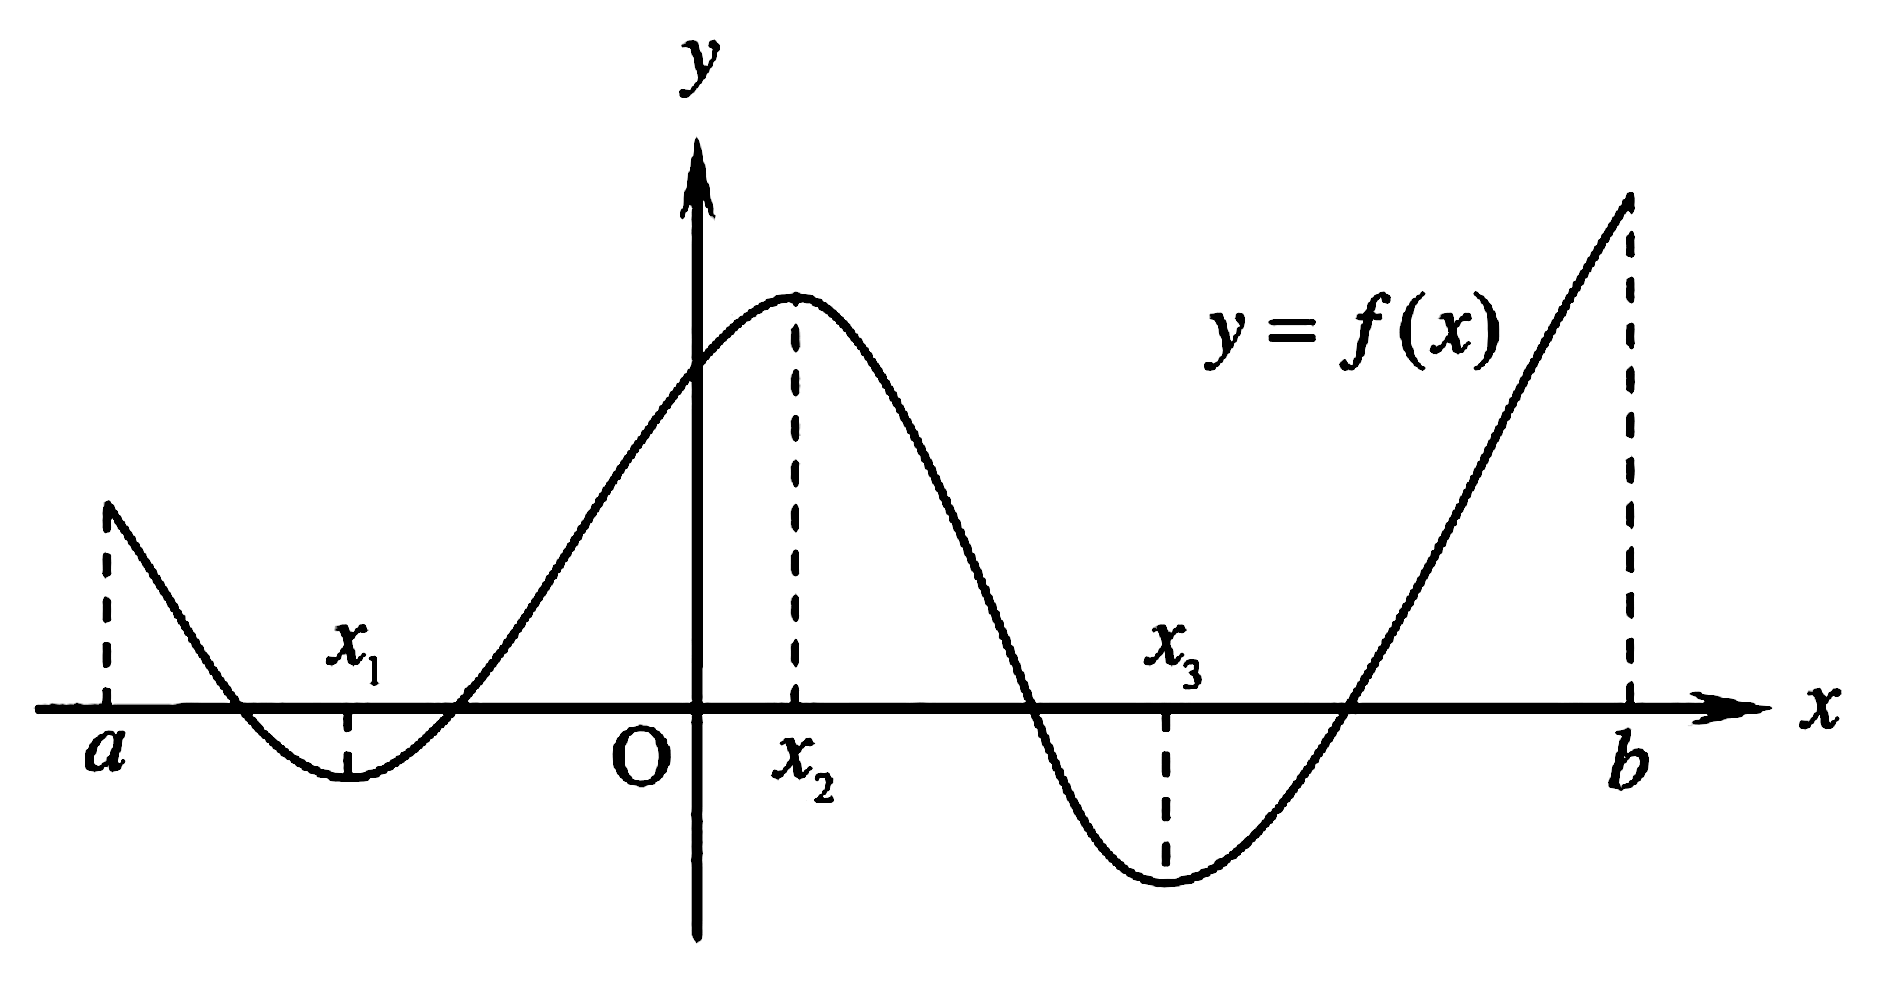
\includegraphics[scale=0.25]{assets/26-8.png}
\end{center}

\begin{center}
    \framebox{
        \parbox[t][1.6cm]{14cm}{ \addvspace{0.4cm} \centering \parbox{13.5cm}{If the function $f(x)$ is continuous in the close interval $[a,
                            b]$, then the function $f(x)$ must have the absolute maximum value and the
                absolute minimum value in the interval $[a, b]$.} }}
\end{center}

The function $f(x)$ that is continuous in the open interval $(a, b)$ may not
have the absolute maximum value and the absolute minimum value. For example,
the function $y = \dfrac{1}{x}$ is continuous in the interval $(0, \infty)$,
but it does not have the absolute maximum value and the absolute minimum value.
Also in the diagram above, if the domain is defined as the open interval $(a,
    b)$, then the function $f(x)$ only has the relative minimum value but not the
absolute minimum value.

From the diagram above, if the function is continuous in the interval $[a, b]$,
we just have to make comparison between all the extreme points and vertices of
the function to find the absolute maximum value and the absolute minimum value
of the function.

\subsection{Practice 4}

\noindent \hspace{1.2em}\textit{Find the absolute maximum value and the absolute minimum value of the following functions (Question 1 to 2):}
\begin{enumerate}
    \item $f(x) = 3x^3 - 9x + 5$, $[-2, 2]$
    \item $f(x) = x^4 - 2x^2 + 5$, $[-2, 3]$
    \item If $x + y = 8$, find the absolute minimum value of $x^2 + y^2$.
    \item A metal wire with a length of $100$cm is bent into a rectangle. Find the width
          and the length of the rectangle so that the area of the rectangle is the
          largest.
\end{enumerate}
\subsection{Exercise 26.4}

\noindent \hspace{1.2em}\textit{Find the absolute maximum value and the absolute minimum value of the following functions (Question 1 to 3):}
\begin{enumerate}
    \item $f(x)=5-36 x+3 x^2+4 x^3$, $[-1,2]$
    \item $f(x)=4 x^2\left(x^2-2\right)$, $[-1,3]$
    \item $f(x)=x^5-5 x^4+5 x^3$, $[0,4]$
    \item A metal wire with a length of $60$cm is bent into a rectangle. Find the width
          and the length of the rectangle so that the area of the rectangle is the
          largest.
    \item A metal wire with a length of $100$cm is cut into two sections. Each section is
          bent into a square. Find the length of these two sections of the wire so that
          the sum of the areas of the two squares is the smallest.
    \item As shown in the diagram below, a trapezium has three sides of length $10$cm.If
          the area of the trapezium is the largest, find the length of the fourth side.
          Hence, find the maximum area of the trapezium.
          \begin{center}
              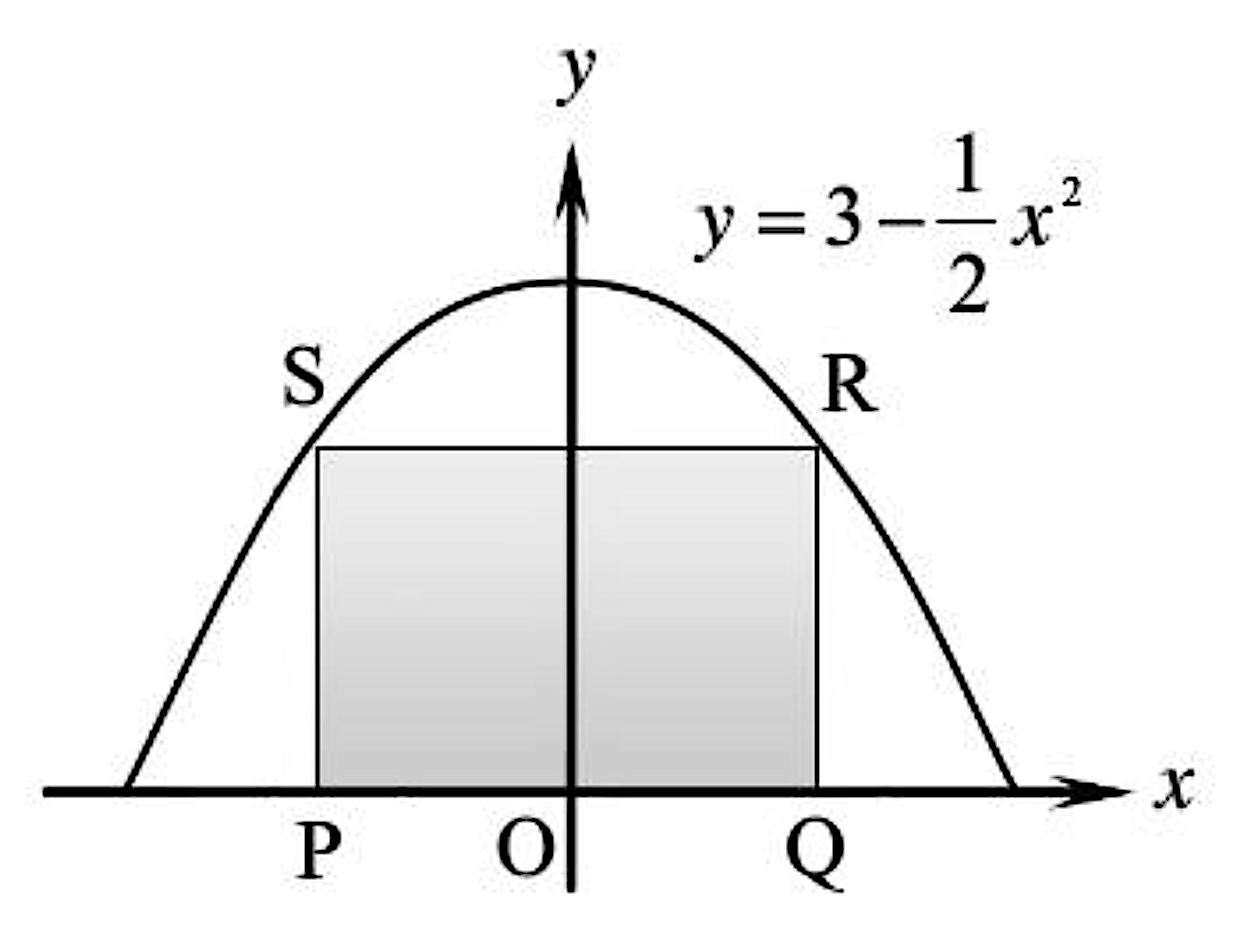
\includegraphics[scale=0.25]{assets/26-9.png}
          \end{center}
    \item A right cone has a slant height of $9$cm. Find the height of the cylinder such
          that the volume of the cylinder is the largest.
    \item A cylinder shaped can with lid has a volume of $250\pi$cm$^3$. Find the bottom
          radius and the height of the can so that the material used is the least.
    \item Split the number 20 into two parts such that one part is 4 times the reciprocal
          of another part, and the the sum of it with with 9 times the reciprocal of
          another part is the smallest.
    \item A metal wire with a length of $150$cm is split into two sections, and they are
          bent into a square and a circle respectively. Find the length of these two
          sections such that the sum of the area of the square and the circle is the
          smallest.
    \item As shown in the diagram below, a window is formed by a rectangle and a
          semicircle. The perimeter of the entire window is 300cm. If the area of the
          window is the largest, find the length of the rectangle. Hence, find the
          maximum area of the window.
          \begin{center}
              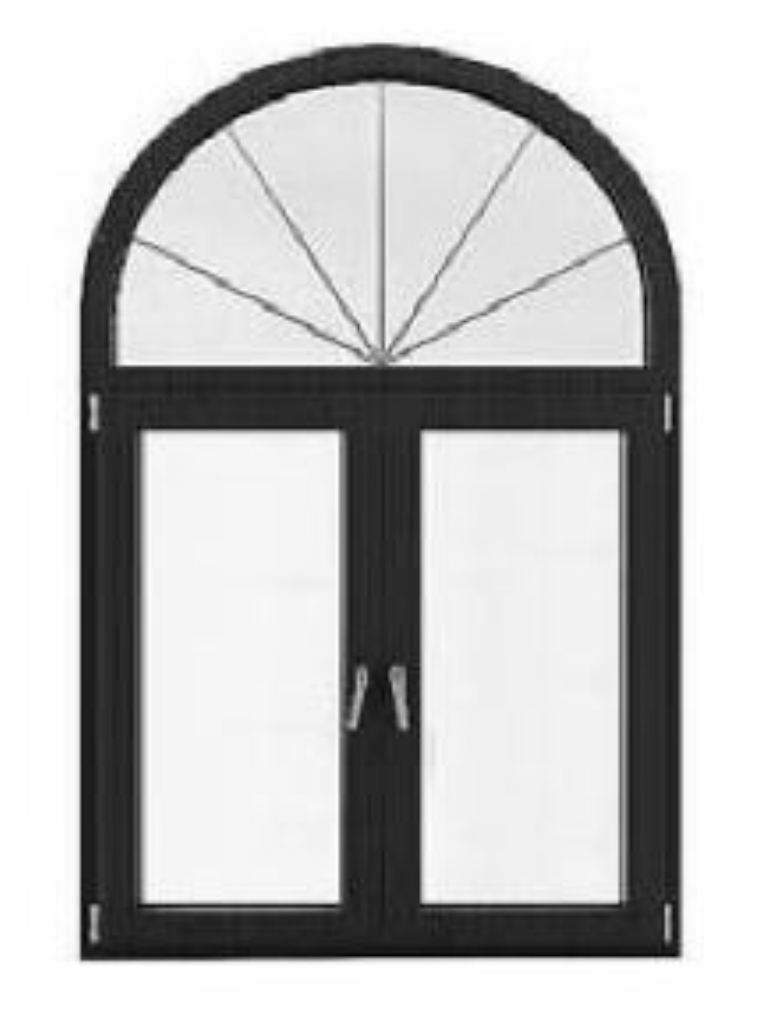
\includegraphics[scale=0.25]{assets/26-10.png}
          \end{center}
    \item In the diagram below, $PQRS$ is a rectangle, the coordinates of $P$ and $Q$ are
          $(-k, 0)$ and $(k, 0)$ respectively, where $k > 0$, and the two points $R$ and
          $S$ are on the curve $y = 3- \dfrac{1}{2}x^2$. Find the value of $k$ such that
          the area of the rectangle is the largest.
          \begin{center}
              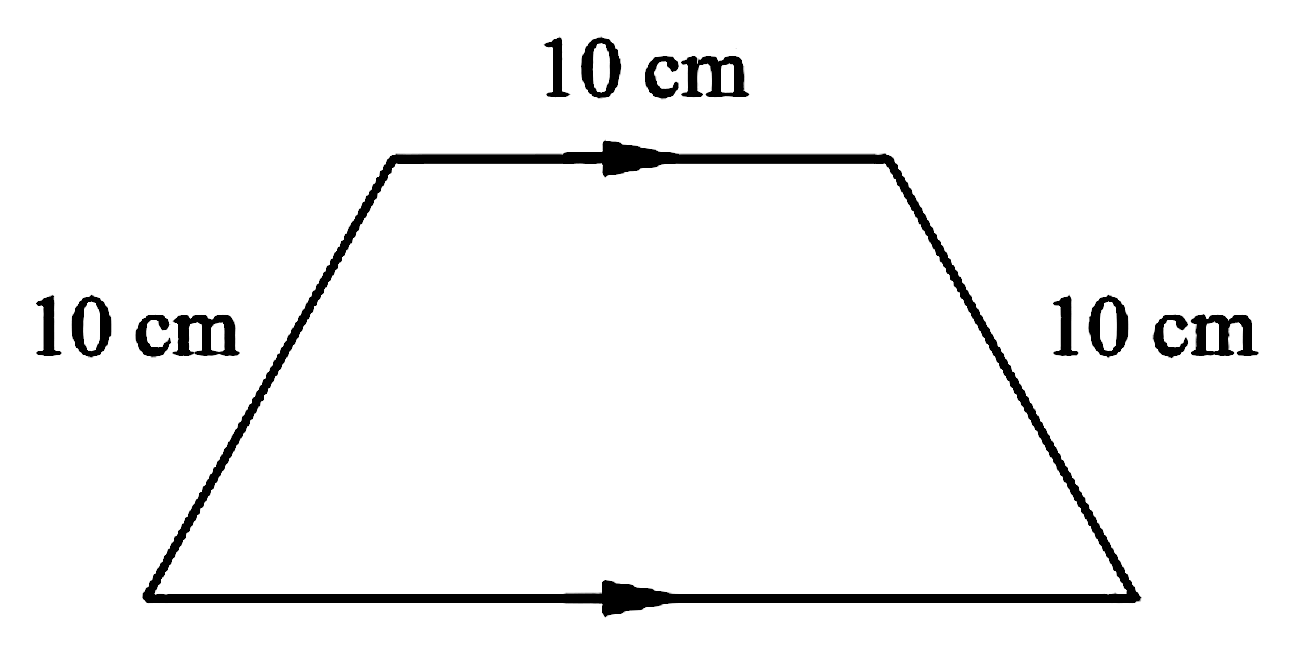
\includegraphics[scale=0.25]{assets/26-11.png}
          \end{center}
\end{enumerate}
\newpage

\section{The Convexity and the Point of Inflection of Functions}

For a curve $y = f(x)$
\begin{enumerate}
    \item In a given interval, if the tangent line of the curve is always above the
          curve, then the curve convex upward in the interval, as shown in the diagram
          below.
          \begin{center}
              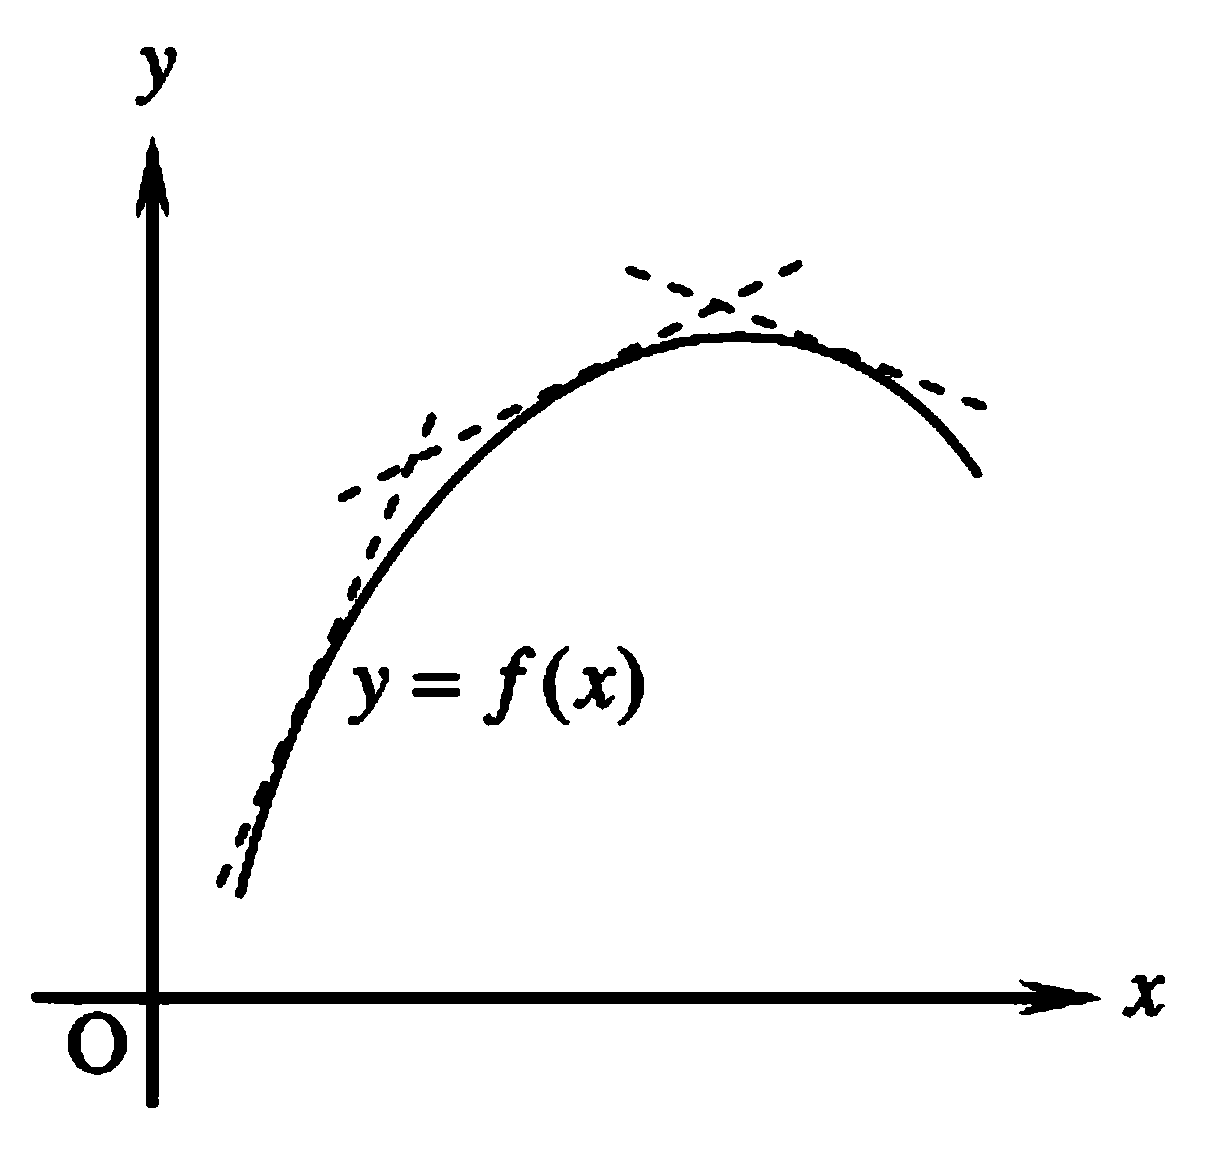
\includegraphics[scale=0.25]{assets/26-12.png}
          \end{center}
    \item In a given interval, if the tangent line of the curve is always below the
          curve, then the curve is convex downward in the interval, as shown in the
          diagram below.
          \begin{center}
              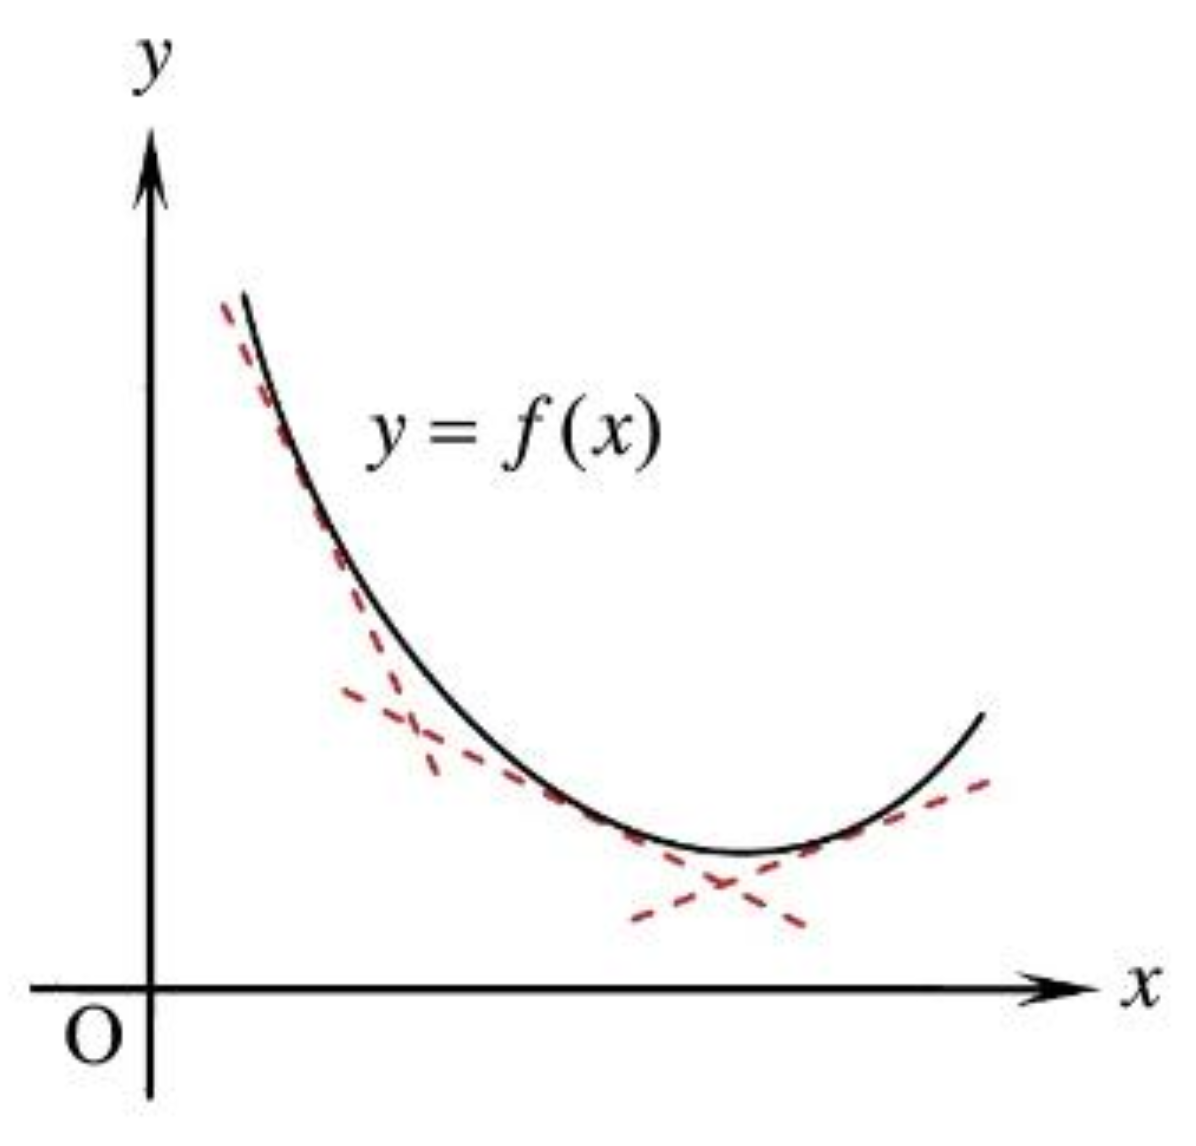
\includegraphics[scale=0.25]{assets/26-13.png}
          \end{center}
\end{enumerate}

If two sides of a point on a curve of a function $y = f(x)$ changes their
concavity, then the demarcation point is called the point of inflection of the
curve.

Now we discuss the way to determine the convexity and the point of inflection
of a function. In the diagram below, the left side of the point $x = x_0$
convex downward, and the right side convex upward.
\begin{center}
    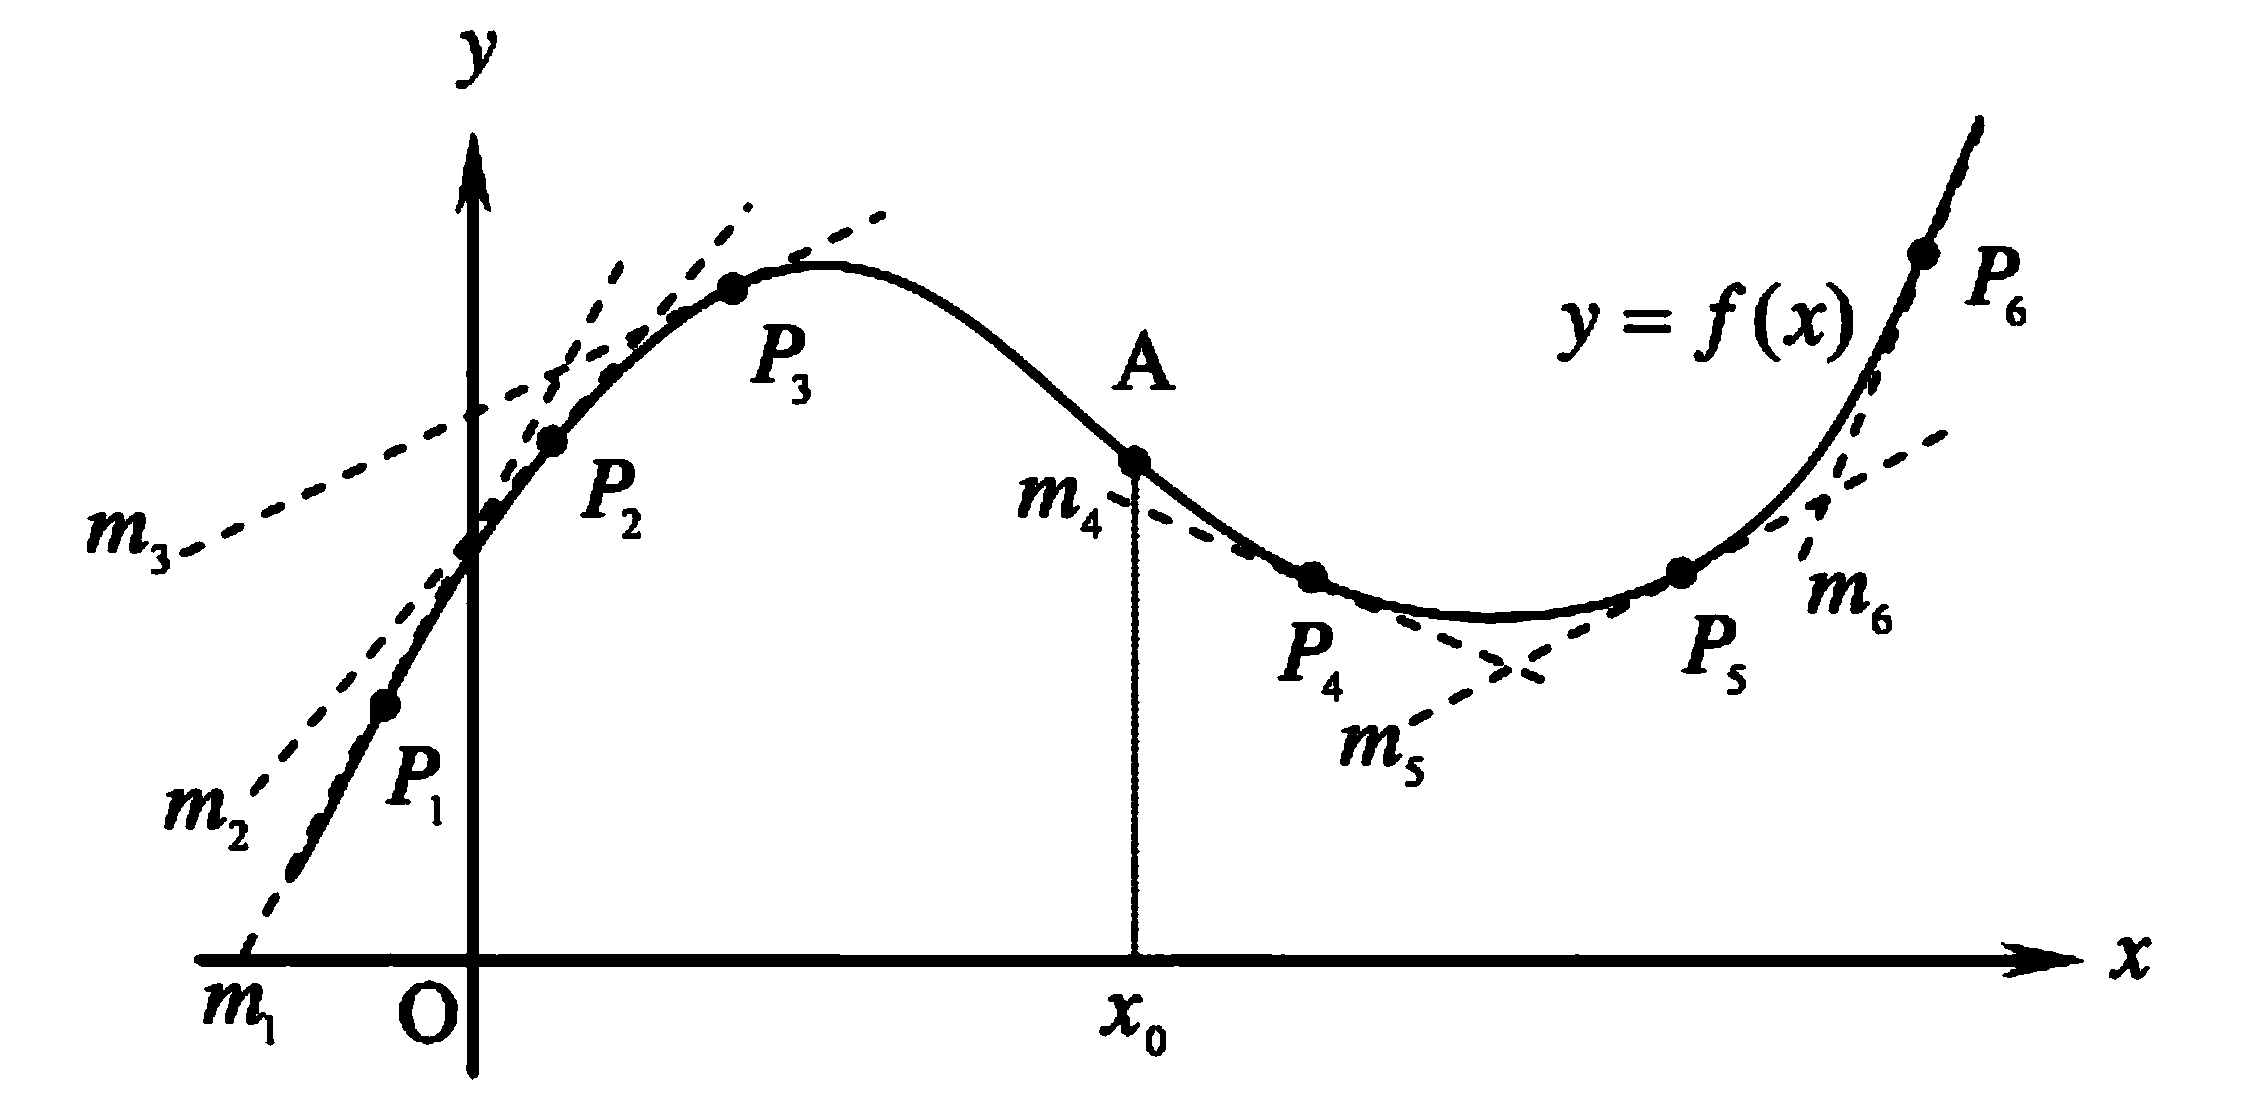
\includegraphics[scale=0.25]{assets/26-14.png}
\end{center}
In the interval $(-\infty, x_0)$ that convex upward, when the tangents to the curve cut the curve at $P_1$, $P_2$, and $P_3$ respectively from left to right, the gradients of the tangent lines $m_1$, $m_2$, and $m_3$ are decreasing, i.e. the gradient of the tangent $f'(x)$ is decreasing.

In the interval $(x_0, \infty)$ that convex downward, when the tangents to the
curve cut the curve at $P_4$, $P_5$, and $P_6$ respectively from left to right,
the gradients of the tangent lines $m_4$, $m_5$, and $m_6$ are increasing, i.e.
the gradient of the tangent $f'(x)$ is increasing.

\newpage
We have the following theorem:
\begin{center}
    \framebox{
        \parbox[t][2.7cm]{14cm}{ \addvspace{0.4cm} \hspace{0.4cm}Let function $f(x)$ has
            second derivative $f''(x)$.
            \begin{itemize}[leftmargin=0.8cm]
                \item \parbox[t]{12.5cm}{If $f''(x) > 0$ in a given interval, then the curve is convex
                          upwards;}
                \item \parbox[t]{12.5cm}{If $f''(x) < 0$ in a given interval, then the curve is convex
                          downwards.}
            \end{itemize} }}
\end{center}

\subsection{Practice 5}
Find the following indefinite integral:
\begin{enumerate}
    \begin{multicols}{2}
        \item $\displaystyle\int\sin2x\cos2x dx$
        \sol{}
        \begin{flalign*}
            I & = \dfrac{1}{2}\int\sin4x dx & \\
              & = -\dfrac{1}{8}\cos4x + C
        \end{flalign*}
        \vfill{}\null{}

        \item $\displaystyle\int\cos^2 2x dx$
        \sol{}
        \begin{flalign*}
            I & = \int\dfrac{1 + \cos 4x}{2} dx                    & \\
              & = \dfrac{1}{2}\int dx + \dfrac{1}{2}\int\cos 4x dx & \\
              & = \dfrac{1}{2}x + \dfrac{1}{8}\sin 4x + C
        \end{flalign*}
    \end{multicols}
    \begin{multicols}{2}
        \item $\displaystyle\int\sin^3 x dx$
        \sol{}
        \begin{flalign*}
            I & = \int\sin^2 x\sin x dx                 & \\
              & = \int(1 - \cos^2 x)\sin x dx           & \\
              & = \int\sin x dx - \int\cos^2 x\sin x dx
        \end{flalign*}
        Let $u = \cos x$, $du = -\sin xdx$.
        \begin{flalign*}
            I & = -\int \cos x dx + \int u^2 du    & \\
              & = -\sin x + \dfrac{1}{3}u^3 + C    & \\
              & = \dfrac{1}{3}\cos^3 x -\sin x + C
        \end{flalign*}

        \item $\displaystyle\int\cos^3 x dx$
        \sol{}
        \begin{flalign*}
            I & = \int\cos^2 x\cos x dx                 & \\
              & = \int(1 - \sin^2 x)\cos x dx           & \\
              & = \int\cos x dx - \int\sin^2 x\cos x dx
        \end{flalign*}
        Let $u = \sin x$, $du = \cos xdx$.
        \begin{flalign*}
            I & = \int \cos x dx - \int u^2 du      & \\
              & = \sin x - \dfrac{1}{3}u^3 + C      & \\
              & = \sin x - \dfrac{1}{3}\sin^3 x + C
        \end{flalign*}
    \end{multicols}
    \begin{multicols}{2}
        \item $\displaystyle\int\tan^4 x\sec^2 x dx$
        \sol{}

        Let $u = \tan x$, $du = \sec^2 xdx$.
        \begin{flalign*}
            I & = \int u^4 du              & \\
              & = \dfrac{u^5}{5} + C       & \\
              & = \dfrac{1}{5}\tan^5 x + C
        \end{flalign*}
        \vfill{}\null{}
        \columnbreak
        \item $\displaystyle\int\tan^4\dfrac{x}{2} dx$
        \sol{}
        \begin{flalign*}
            I & = \int\tan^2\dfrac{x}{2}\tan^2\dfrac{x}{2} dx                             & \\
              & = \int\left(\sec^2\dfrac{x}{2} - 1\right)\tan^2\dfrac{x}{2} dx            & \\
              & = \int\sec^2\dfrac{x}{2}\tan^2\dfrac{x}{2} dx - \int\tan^2\dfrac{x}{2} dx
        \end{flalign*}
        Let $u = \tan\dfrac{x}{2}$, $du = \dfrac{1}{2}\sec^2\dfrac{x}{2}dx$.
        \begin{flalign*}
            I & = 2\int u^2 du - \int \tan^2\dfrac{x}{2} dx                     & \\
              & = \dfrac{2u^3}{3} - \int \left(\sec^2\dfrac{x}{2} - 1\right) dx & \\
              & = \dfrac{2u^3}{3} - \int \sec^2\dfrac{x}{2} dx + \int dx        & \\
              & = \dfrac{2}{3}\tan^3\dfrac{x}{2} - 2\tan\dfrac{x}{2} + x + C
        \end{flalign*}
    \end{multicols}
\end{enumerate}
\subsection{Practice 26.5}
\noindent \hspace{1.2em}\textit{Find the coordinates of the points of inflection of the following functions (Question 1 to 3):}
\begin{enumerate}
    \item $f(x)=x^3-6 x+4$
    \item $f(x)=x^3(4-x)$
    \item $f(x)=x^{\frac{7}{3}}$
\end{enumerate}

\noindent \hspace{1.2em}\parbox{\textwidth-1.2em}{\textit{Find the intervals where the following functions
        are convex up or convex down, and find the points of inflection of the
        functions (Question 4 to 6):}}
\begin{enumerate}[resume]
    \item $f(x)=-(x-2)^3$
    \item $f(x)=2 x^3-3 x^2-36 x+25$
    \item $f(x)=x^4-2 x^3+1$
\end{enumerate}

\noindent \hspace{1.2em}\parbox{\textwidth-1.2em}{\textit{Find the extreme values, the coordinates of the
        points of inflection, and the intervals where the following functions are
        convex up or convex down (Question 7 to 8):}}
\begin{enumerate}[resume]
    \item $f(x)=x(6-2 x)^2$
    \item $f(x)=-\dfrac{2}{1+x^2}$
\end{enumerate}

\section{Curve Sketching}

Having learnt the derivatives, we can use the concepts of the increasing and
decreasing of a function, the convexity and the point of inflection of a
function to sketch the curve of a function in a rather accurate way. Listed
below are the steps to sketch the curve of a function:
\begin{enumerate}
    \item Find the point of intersections of the curve with the axes;
    \item Solve the equation $f'(x) = 0$, and determine the intervals where the function
          is increasing or decreasing and the extreme values;
    \item Solve the equation $f''(x) = 0$, and determine the intervals where the curve is
          convex upward or convex downward and the points of inflection;
    \item Draw the curve according to the above information.
\end{enumerate}
The steps above are not necessarily to be followed in the order listed, and can be adjusted according to the actual situation.

\subsection{Practice 6}

Sketch the graph of the function $f(x) = x^3 - 3x^2 + 2$.
\subsection{Exercise 26.6}

Sketch the graph of the following functions (Question 1 to 3):

\begin{enumerate}
      \item $f(x)=\dfrac{1}{3} x^3-\dfrac{1}{2} x^2-2 x$
            \sol{}
            \vspace{-1cm}
            \begin{multicols}{2}
                  \begin{flalign*}
                        f(0)                                   & = 0                                                                     & \\
                        \dfrac{1}{3}x^3 - \dfrac{1}{2}x^2 - 2x & = 0                                                                     & \\
                        2x^3 - 3x^2 - 12x                      & = 0                                                                     & \\
                        x(2x^2 - 3x - 12)                      & = 0                                                                     & \\
                        x                                      & = 0 \text{ or } 2x^2 - 3x - 12 = 0                                      & \\
                                                               & = 0 \text{ or } x = \dfrac{3 \pm \sqrt{105}}{4}                           \\
                        f'(x)                                  & = x^2 - x - 2                                                           & \\
                        f''(x)                                 & = 2x - 1                                                                & \\
                        x^2 - x - 2                            & = 0                                                                     & \\
                        (x - 2)(x + 1)                         & = 0                                                                     & \\
                        x                                      & = 2 \text{ or } x = -1                                                  & \\
                        f(2)                                   & = \dfrac{1}{3}\left(2\right)^3 - \dfrac{1}{2}\left(2\right)^2 - 2(2)      \\
                                                               & = \dfrac{8}{3} - 2 - 4                                                    \\
                                                               & = -\dfrac{10}{3}                                                          \\
                        f(-1)                                  & = \dfrac{1}{3}\left(-1\right)^3 - \dfrac{1}{2}\left(-1\right)^2 - 2(-1)   \\
                                                               & = -\dfrac{1}{3} - \dfrac{1}{2} + 2                                        \\
                                                               & = \dfrac{7}{6}                                                            \\
                        f''(2)                                 & = 3 > 0                                                                   \\
                        f''(-1)                                & = -3 < 0
                  \end{flalign*}

                  \begin{flalign*}
                        2x - 1                     & = 0                                                                                                              & \\
                        x                          & = \dfrac{1}{2}                                                                                                   & \\
                        f\left(\dfrac{1}{2}\right) & = \dfrac{1}{3}\left(\dfrac{1}{2}\right)^3 - \dfrac{1}{2}\left(\dfrac{1}{2}\right)^2 - 2\left(\dfrac{1}{2}\right)   \\
                                                   & = \dfrac{1}{24} - \dfrac{1}{8} - 1                                                                                 \\
                                                   & = -\dfrac{13}{12}
                  \end{flalign*}
                  $x$-intercepts: $\left(0, 0\right)$, $\left(\dfrac{3 - \sqrt{105}}{4}, 0\right)$, $\left(\dfrac{3 + \sqrt{105}}{4}, 0\right)$

                  \noindent $y$-intercept: $(0, 0)$

                  \noindent Relative maximum: $\left(-1, \dfrac{7}{6}\right)$

                  \noindent Relative minimum: $\left(2, -\dfrac{10}{3}\right)$

                  \noindent Points of inflection: $\left(\dfrac{1}{2}, -\dfrac{13}{12}\right)$

                  \noindent Convex up: $\left(-\infty, \dfrac{1}{2}\right)$

                  \noindent Convex down: $\left(\dfrac{1}{2}, \infty\right)$
            \end{multicols}
            \vfill\null
            \begin{center}
                  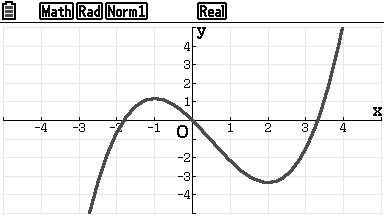
\includegraphics[scale=0.7]{26-graph2.png}
            \end{center}
            \vfill\null
            \newpage

      \item $f(x)=x^4-32 x+10$
            \sol{}
            \vspace{-0.6cm}
            \begin{vwcol}[widths={0.3,0.7},justify=flush,rule=0pt,indent=1em]
                  \begin{flalign*}
                        f(0)      & = 10               & \\
                        f'(x)     & = 4x^3 - 32        & \\
                        f''(x)    & = 12x^2            & \\
                        4x^3 - 32 & = 0                & \\
                        x         & = 2                & \\
                        f(2)      & = 2^4 - 32(2) + 10   \\
                                  & = -38              & \\
                        f''(2)    & = 48 > 0           & \\
                        12x^2     & = 0                & \\
                        x         & = 0                & \\
                        f(0)      & = 10
                  \end{flalign*}
                  y-intercept: $(0, 10)$

                  \noindent Relative minimum: $(2, -38)$

                  \noindent Points of inflection: $(0, 10)$

                  \noindent Convex down: $(-\infty, \infty)$
                  \newpage
                  \vspace*{2cm}
                  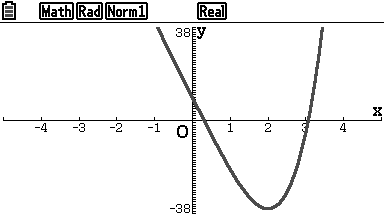
\includegraphics[scale=0.7]{26-graph3.png}
            \end{vwcol}

      \item $f(x)=(x-1)^3(x-2)$
            \sol{}
            \vspace{-1cm}
            \begin{multicols}{2}
                  \begin{flalign*}
                        f(0)                         & = 2                                                     & \\
                        (x-1)^3(x-2)                 & = 0                                                       \\
                        x                            & = 1 \text{ or } x = 2                                     \\
                        f'(x)                        & = 3(x-1)^2(x-2) + (x-1)^3                                 \\
                                                     & = (x-1)^2(3x-6+x-1)                                       \\
                                                     & = (x-1)^2(4x-7)                                           \\
                        f''(x)                       & = 2(x-1)(4x-7) + (x-1)^2(4)                               \\
                                                     & = 2(x-1)(4x-7+2x-2)                                       \\
                                                     & = 2(x-1)(6x-9)                                            \\
                                                     & = 6(x-1)(2x-3)                                            \\
                        (x-1)^2(4x-7)                & = 0                                                       \\
                        x                            & = 1 \text{ or } x = \dfrac{7}{4}                          \\
                        f(1)                         & = 0                                                       \\
                        f\left(\dfrac{7}{4}\right)   & = \left(\dfrac{3}{4}\right)^3\left(-\dfrac{1}{4}\right)   \\
                                                     & = -\dfrac{27}{256}                                        \\
                        f''(1)                       & = 0                                                       \\
                        f''\left(\dfrac{7}{4}\right) & = 6\left(\dfrac{3}{4}\right)\left(\dfrac{7}{2}-3\right)   \\
                                                     & = \dfrac{9}{4} > 0                                      &
                  \end{flalign*}

                  \begin{flalign*}
                        6(x-1)(2x-3)               & = 0                                                     \\
                        x                          & = 1 \text{ or } x = \dfrac{3}{2}                        \\
                        f(1)                       & = 0                                                     \\
                        f\left(\dfrac{3}{2}\right) & = \left(\dfrac{1}{2}\right)^3\left(-\dfrac{1}{2}\right) \\
                                                   & = -\dfrac{1}{16}
                  \end{flalign*}
                  $x$-intercepts: $(1, 0)$, $\left(2, 0\right)$

                  \noindent $y$-intercept: $(0, 2)$

                  \noindent Relative minimum: $\left(\dfrac{7}{4}, -\dfrac{27}{256}\right)$

                  \noindent Points of inflection: $\left(1, 0\right)$, $\left(\dfrac{3}{2}, -\dfrac{1}{16}\right)$

                  \noindent Convex downwards: $\left(-\infty, 1\right)$, $\left(\dfrac{3}{2}, \infty\right)$

                  \noindent Convex upwards: $\left(1, \dfrac{3}{2}\right)$
            \end{multicols}
            \begin{center}
                  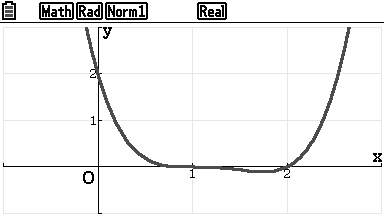
\includegraphics[scale=0.6]{26-graph4.png}
            \end{center}

      \item Given the function $f(x) = x^3(4-x)$.
            \begin{enumerate}
                  \begin{multicols}{2}
                        \item Find the extreme values and the intervals of increasing and decreasing of
                        $f(x)$. \sol{}
                        \begin{flalign*}
                              f(x)        & = 4x^3 - x^4      \\
                              f'(x)       & = 12x^2 - 4x^3    \\
                                          & = 4x^2(3 - x)     \\
                              4x^2(3 - x) & = 0               \\
                              x = 0       & \text{ or } x = 3 \\
                              f(0)        & = 0               \\
                              f(3)        & = 27              \\
                              f''(x)      & = 24x - 12x^2     \\
                              f''(0)      & = 0               \\
                              f''(3)      & = 36 > 0
                        \end{flalign*}
                        $\therefore$ Relative maximum: $f(3) = 27$

                        In the interval $(-\infty, 0)$, $f'(x) > 0$, so $f(x)$ is increasing in the
                        interval $(-\infty, 0]$.

                        In the interval $(0, 3)$, $f'(x) > 0$, so $f(x)$ is increasing in the interval
                        $[0, 3]$.

                        In the interval $(3, \infty)$, $f(x)$ is decreasing in the interval $[3,
                                          \infty)$. \columnbreak

                                                \item Find the points of inflection and the intervals of convexity and concavity of
                                          $f(x)$. \sol{}
                                                \begin{flalign*}
                                                      24x - 12x^2 & = 0               \\
                                                      x(2 - x)    & = 0               \\
                                                      x = 0       & \text{ or } x = 2 \\
                                                      f(0)        & = 0               \\
                                                      f(2)        & = 16
                                                \end{flalign*}
                                          $\therefore$ Point of inflection: $(2, 16)$, $(0, 0)$

                                                In the interval $(-\infty, 0)$, $f''(x) < 0$, so $f(x)$ is convex upward in the
                                                interval $(-\infty, 0]$.

                        In the interval $(0, 2)$, $f''(x) < 0$, so $f(x)$ is convex upward in the
                        interval $[0, 2]$.

                        In the interval $(2, \infty)$, $f''(x) > 0$, so $f(x)$ is convex downward in
                        the interval $[2, \infty)$.
                  \end{multicols}

                  \item Hence, sketch the graph of $f(x)$. \sol{}
                        \begin{center}
                              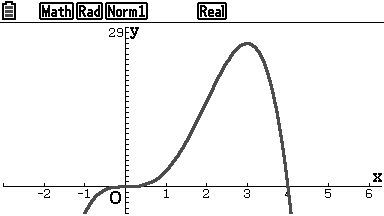
\includegraphics[scale=0.6]{26-graph5.png}
                        \end{center}
            \end{enumerate}
\end{enumerate}

\section{Rate of Change and Related Rate of Change}

The derivative of the function $y = f(x)$ at the point $x = x_0$ is known as
the rate of change of the dependent value $y$ with respect to the independent
value $x$ at the point $x = x_0$. For example, $\dfrac{d y}{d x} = 3$ means
that when $x$ increases by $1$ unit, $y$ increases by $3$ units, i.e. $y$ and
$x$ are both changing, and they are changing in the ratio of $3:1$.

The same can be said that the derivative of the area function $A = A(t)$ at the
time $t = t_0$ is the rate of change of the area with respect to the time at
the time $t = t_0$. When the rate of change of the area at $t = t_0$ is
$\dfrac{d A}{d t} = 4$cm$^2$/s, it means that the area is increasing in the
rate of 4 square centimetres per second; while $\dfrac{d A}{d t} = -4$cm$^2$/s
means that the area is decreasing in the rate of 4 square centimetres per
second.

If multiple variables are correlated by a specific relationship, these
variables are all changing with respect to time, then there must be some kind
of bonds between their respective rate of changes. This relationship between
the rate of changes is called the related rate of change. If $y = f(x)$ is the
function of $x$, and $x$ changes with respect to $t$, then since $y$ is
changing with respect to $x$, $y$ is also changing with respect to $t$. In
other words, $y$ is also a function of the time $t$. HEnce, from the chain
rule, we can obtain the following relationship:
\begin{cequation}
    \dfrac{dy}{dt} = \dfrac{dy}{dx} \cdot \dfrac{dx}{dt}
\end{cequation}
i.e. the rate of change of $y$ is correlated to the rate of change of $x$.

\subsection{Practice 7}
\begin{enumerate}
      \begin{multicols}{2}
            \item A drop of ink gradually spread after being dropped onto a piece of paper. At
            $t$ seconds, its area is $A = \left(3t^2 + \dfrac{1}{5}t + 2\right)$mm$^2$.
            Find the rate of change of the ink spread at $t = 2$ second. \sol{}
            \begin{flalign*}
                  \dfrac{dA}{dt} & = 6t + \dfrac{1}{5}
            \end{flalign*}
            When $t = 2$,
            \begin{flalign*}
                  \dfrac{dA}{dt} & = 6(2) + \dfrac{1}{5}      \\
                                 & = 12 + \dfrac{1}{5}        \\
                                 & = \dfrac{61}{5}            \\
                                 & = 12.2\text{mm}^2\text{/s}
            \end{flalign*}
            \vfill\null

            \item The radius of a sphere increases at a rate of $3$cm/s. When the radius is
            $5$cm, find the rate of change of the surface area of the sphere. \sol{}
            \begin{flalign*}
                  \dfrac{dr}{dt} & = 3\text{cm/s}                      \\
                  A              & = 4\pi r^2                          \\
                  \dfrac{dA}{dr} & = 8\pi r                            \\
                  \dfrac{dA}{dt} & = \dfrac{dA}{dr}\cdot\dfrac{dr}{dt} \\
                                 & = 8\pi r\cdot 3\text{cm/s}          \\
                                 & = 24\pi r\text{cm}^2\text{/s}
            \end{flalign*}
            When $r = 5$,
            \begin{flalign*}
                  \dfrac{dA}{dt} & = 24\pi(5)\text{cm}^2\text{/s} \\
                                 & = 120\pi\text{cm}^2\text{/s}
            \end{flalign*}
      \end{multicols}
\end{enumerate}
\subsection{Exercise 26.7}
\begin{enumerate}
    \item Water is poured into a container, the relationship between the volume of the
          water and the time is $V = (2t^2 + 3t)$cm$^3$. WHen $t = 3$s, find the rate of
          change of the volume of the water.
    \item One throws a piece of stone into the water. The radius of the ripple on the
          water surface caused by the stone is increasing at a rate of $0.1$m/s. When the
          radius is $1$m, find the rate of change of the area of the ripple.
    \item The side length of a square is increasing at a rate of $3$cm per second. When
          the side length is $15$cm, find the rate of change of its area.
    \item A cube expanded after being heated, the rate of change of its side length is
          $5$cm/s. When the side length is $4$cm, find the rate of change of its area.
    \item The radius of a sphere increases by 1cm per second. When the radius is 3cm,
          find the rate of change of its volume.
    \item The area of a circle increases by 5cm$^2$ per minute. When the circumference of
          the circle is 40cm find the rate of change of its radius.
    \item The volume of a sphere decreases at a rate of $12\pi$cm$^3$ per minute. When
          the radius of the sphere is 6cm, find the rate of change of its radius and
          surface area.
    \item The surface area of a sphere increase at a rate of $10$cm$^2$/s. When its
          radius is 5cm, find the rate of change of its radius and volume.
    \item Water is poured into the cone shaped container as shown in the diagram below,
          the rate of rising of the water surface is $1$cm per second. When the depth of
          the water is $2m$, find the rate of change of the water volume.
          \begin{center}
              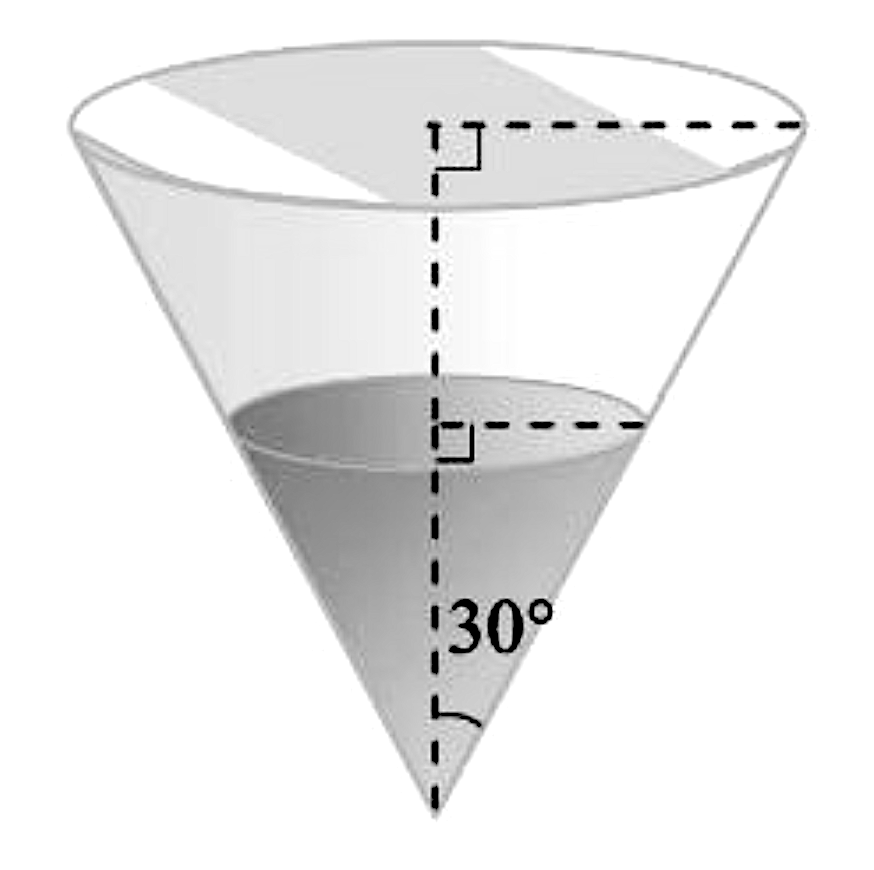
\includegraphics[scale=0.25]{assets/26-15.png}
          \end{center}
    \item The radius $r$ of a solid cylinder decreases by $0.04$cm per second, its height
          constantly equal to 20cm. When the radius is 2cm, find the rate of change of
          the surface area of the cylinder.
    \item Given the function $y = x^3 + 10$. When the rate of change of $y$ is 27 times
          the rate of change of $x$, find the value of $x$.
    \item Water is poured ito a cone shaped container facing downwards with a height of
          18m and a base radius of 24m. WHen the height of the water is 6m, find the rate
          of rising of the water surface.
\end{enumerate}


\section{Approximate Calculation}

In the previous chapter, we have learnt that the derivative of the function $y
    = f(x)$ is
\begin{cequation}
    \dfrac{dy}{dx} = \lim_{\Delta x \to 0}\dfrac{\Delta y}{\Delta x} = \lim_{\Delta x \to 0}\dfrac{f(x + \Delta x) - f(x)}{\Delta x}
\end{cequation}
From the definition of limit, we know that when $\Delta x$ is small enough,
\begin{cequation}
    \dfrac{\Delta y}{\Delta x} = \dfrac{\Delta y}{\Delta x} \approx \dfrac{f(x + \Delta x) - f(x)}{\Delta x}
\end{cequation}
Hence,
\begin{center}
    \framebox{
        \parbox[t][1.2cm]{9cm}{ \addvspace{0.25cm} \centering $\Delta y \approx
                \dfrac{dy}{dx}\Delta x$ }}
\end{center}
or $f(x + \Delta x) - f(x) \approx f'(x)\Delta x$, i.e.
\begin{center}
    \framebox{
        \parbox[t][1.2cm]{9cm}{ \addvspace{0.45cm} \centering $f(x + \Delta x) \approx f(x)
                + f'(x)\Delta x$ }}
\end{center}

The expression above is a simple formula for approximate calculation that can
be used to find the approximate value of a function.
\begin{center}
    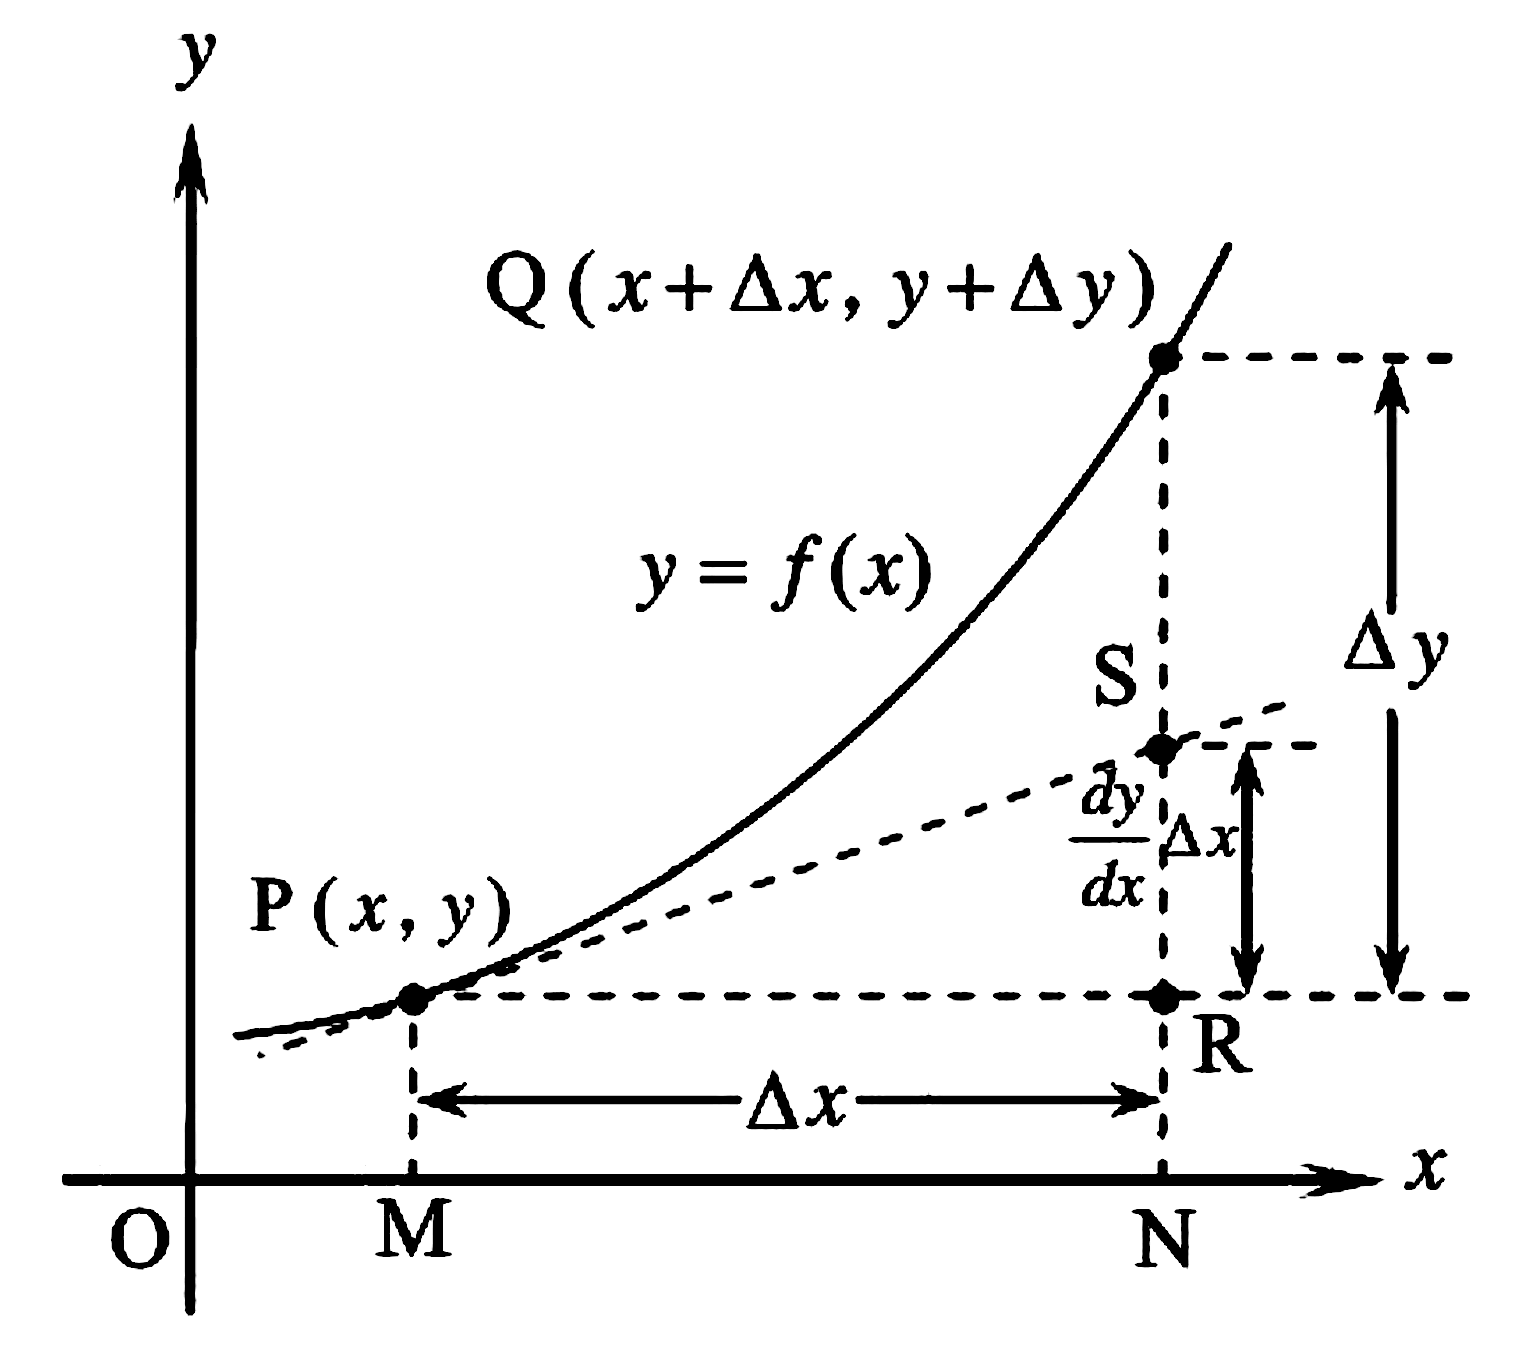
\includegraphics[scale=0.25]{assets/26-16.png}
\end{center}

\subsection{Practice 8}

\begin{enumerate}
      \item The side length of a cube increases from 1cm to $1.01$cm, how much does its
            surface area increase approximately? \sol{}

            Let the side length be $x$cm, then the surface area is $A = 6x^2$.
            \begin{flalign*}
                  \dfrac{dA}{dx}             & = 12x                  & \\
                  \dfrac{\Delta A}{\Delta x} & \approx \dfrac{dA}{dx} & \\
                  \Delta A                   & \approx 12x\Delta x
            \end{flalign*}
            \vspace{-0.8em}
            When $x = 1$cm, $\Delta x = 0.01$cm,
            \begin{flalign*}
                  \Delta A & \approx 12(1)(0.01) = 0.12\text{cm}^2 &
            \end{flalign*}
            $\therefore$ The surface area increases by $0.12$cm$^2$ approximately.

            \begin{multicols}{2}
                  \item After a metal ball was heated, its radius had increased form 4cm to $4.01$cm.
                  Find the approximate increment of its volume and surface area. \sol{}

                  Let the radius be $r$cm, then the volume is $V = \dfrac{4}{3}\pi r^3$ and the
                  surface area is $A = 4\pi r^2$.
                  \begin{flalign*}
                        \dfrac{dV}{dr}             & = 4\pi r^2               & \\
                        \dfrac{dA}{dr}             & = 8\pi r                 & \\
                        \dfrac{\Delta V}{\Delta r} & \approx \dfrac{dV}{dr}   & \\
                        \Delta V                   & \approx 4\pi r^2\Delta r & \\
                        \dfrac{\Delta A}{\Delta r} & \approx \dfrac{dA}{dr}   & \\
                        \Delta A                   & \approx 8\pi r\Delta r
                  \end{flalign*}
                  When $r = 4$cm, $\Delta r = 0.01$cm,
                  \begin{flalign*}
                        \Delta V & \approx 4\pi(4)^2(0.01) & \\
                                 & = 0.64\pi\text{cm}^3    & \\
                        \Delta A & \approx 8\pi(4)(0.01)   & \\
                                 & = 0.32\pi\text{cm}^2
                  \end{flalign*}
                  $\therefore$ The volume increases by $0.64\pi$cm$^3$ and the surface area increases by $0.32\pi$cm$^2$ approximately.
                  \columnbreak
                  \item Find the approximate value of $\sqrt{15}$. \sol{}
                  \begin{flalign*}
                        f(x)                       & = \sqrt{x}                           & \\
                        f'(x)                      & = \dfrac{1}{2\sqrt{x}}               & \\
                        \dfrac{\Delta f}{\Delta x} & \approx \dfrac{df}{dx}               & \\
                        \Delta f                   & \approx \dfrac{1}{2\sqrt{x}}\Delta x
                  \end{flalign*}
                  When $x = 16$, $\Delta x = -1$,
                  \begin{flalign*}
                        \Delta f & \approx \dfrac{1}{2\sqrt{16}}(-1) & \\
                                 & = -\dfrac{1}{8}                   & \\
                                 & = -0.125
                  \end{flalign*}
                  $\therefore$ $\sqrt{15} \approx \sqrt{16} - 0.125 = 3.875$.
            \end{multicols}
\end{enumerate}


\subsection{Exercise 26.8}
\begin{enumerate}
      \begin{multicols}{2}
            \item The side length of a square increased from 4cm to $4.001$cm, how much does its
            area increase approximately? \sol{}

            Let $x$ be the side length of the cube, then the area of the cube is $A = x^2$.
            \begin{flalign*}
                  \dfrac{dA}{dx}             & = 2x                            & \\
                  \dfrac{\Delta A}{\Delta x} & \approx \dfrac{dA}{dx} \Delta x & \\
                  \Delta A                   & \approx 2x \Delta x
            \end{flalign*}
            When $x = 4$, $\Delta x = 0.001$,
            \begin{flalign*}
                  \Delta A & \approx 2(4)(0.001) & \\
                           & = 0.008\text{cm}^2
            \end{flalign*}
            $\therefore$ The area of the square increases by $0.008\text{cm}^2$ approximately.

            \item The radius of a circle increases from 3cm to $3.01$cm, find the approximate
            increment of its area. \sol{}

            Let $r$ be the radius of the circle, then the area of the circle is $A = \pi
                  r^2$.
            \begin{flalign*}
                  \dfrac{dA}{dr}             & = 2\pi r                        & \\
                  \dfrac{\Delta A}{\Delta r} & \approx \dfrac{dA}{dr} \Delta r & \\
                  \Delta A                   & \approx 2\pi r \Delta r
            \end{flalign*}
            When $r = 3$, $\Delta r = 0.01$,
            \begin{flalign*}
                  \Delta A & \approx 2\pi(3)(0.01) & \\
                           & = 0.06\pi\text{cm}^2
            \end{flalign*}
            $\therefore$ The area of the circle increases by $0.06\pi\text{cm}^2$
            approximately.
      \end{multicols}

      \begin{multicols}{2}
            \item The radius of a sphere decrease from 3cm to $2.98$cm, find the approximate
            decrement of its volume. \sol{}

            Let $r$ be the radius of the sphere, then the volume of the sphere is $V =
                  \dfrac{4}{3}\pi r^3$.
            \begin{flalign*}
                  \dfrac{dV}{dr}             & = 4\pi r^2                      & \\
                  \dfrac{\Delta V}{\Delta r} & \approx \dfrac{dV}{dr} \Delta r & \\
                  \Delta V                   & \approx 4\pi r^2 \Delta r
            \end{flalign*}
            When $r = 3$, $\Delta r = -0.02$,
            \begin{flalign*}
                  \Delta V & \approx 4\pi(3)^2(-0.02) & \\
                           & = -0.72\pi\text{cm}^3
            \end{flalign*}
            $\therefore$ The volume of the sphere decreases by $0.72\pi\text{cm}^3$
            approximately.

            \item Let $y = 3x^5$. If $x$ is decreased by $0.2\%$, how many percent does $y$
            decrease approximately? \sol{}
            \begin{flalign*}
                  \dfrac{dy}{dx}             & = 15x^4                         & \\
                  \dfrac{\Delta y}{\Delta x} & \approx \dfrac{dy}{dx} \Delta x & \\
                  \Delta y                   & \approx 15x^4 \Delta x
            \end{flalign*}
            When $\Delta x = -0.002x$,
            \begin{flalign*}
                  \Delta y                         & \approx 15x^4(-0.002x)                & \\
                                                   & = -0.03x^5                            & \\
                  \dfrac{\Delta y}{y} \times 100\% & = \dfrac{-0.03x^5}{3x^5} \times 100\% & \\
                                                   & = -1\%
            \end{flalign*}
            $\therefore$ $y$ decreases by $1\%$ approximately.
      \end{multicols}

      \item If the side length of a cube increases by $1\%$, how many percent does its
            volume increase approximately? \sol{}

            Let $x$ be the side length of the cube, then the volume of the cube is $V =
                  x^3$.
            \begin{flalign*}
                  \dfrac{dV}{dx}             & = 3x^2                          & \\
                  \dfrac{\Delta V}{\Delta x} & \approx \dfrac{dV}{dx} \Delta x & \\
                  \Delta V                   & \approx 3x^2 \Delta x
            \end{flalign*}
            When $\Delta x = 0.01x$,
            \begin{flalign*}
                  \Delta V                         & \approx 3x^2(0.01x)                 & \\
                                                   & = 0.03x^3                           & \\
                  \dfrac{\Delta V}{V} \times 100\% & = \dfrac{0.03x^3}{x^3} \times 100\% & \\
                                                   & = 3\%
            \end{flalign*}
            $\therefore$ The volume of the cube increases by $3\%$ approximately.

      \item Let the surface area of a solid right cylinder with a height of 16cm and a
            radius of $r$cm be $A$.
            \begin{enumerate}
                  \item Prove that $\dfrac{dA}{dr} = 4\pi(r+8)$. \prooff{}
                        \begin{flalign*}
                              A              & = 2\pi r^2 + 2\pi rh    &      \\
                                             & = 2\pi r^2 + 2\pi r(16) &      \\
                                             & = 2\pi r^2 + 32\pi r    &      \\
                              \dfrac{dA}{dr} & = 4\pi r + 32\pi        &      \\
                                             & = 4\pi(r+8)             & \qed
                        \end{flalign*}

                  \item If the height of the right cylinder remains the same, using the result obtained
                        from (a), find, when the radius of the right cylinder increases from 4cm to
                        $4.02$cm, the approximate increment of its surface area. \sol{}
                        \begin{flalign*}
                              \dfrac{dA}{dr}             & = 4\pi(r+8)                     & \\
                              \dfrac{\Delta A}{\Delta r} & \approx \dfrac{dA}{dr} \Delta r & \\
                              \Delta A                   & \approx 4\pi(r+8) \Delta r
                        \end{flalign*}
                        When $r = 4$, $\Delta r = 0.02$,
                        \begin{flalign*}
                              \Delta A & \approx 4\pi(4+8)(0.02) & \\
                                       & = 0.96\pi\text{cm}^2
                        \end{flalign*}
                        $\therefore$ The surface area of the right cylinder increases by $0.96\pi\text{cm}^2$ approximately.
            \end{enumerate}
            \vfill\null

      \item If $y = \dfrac{1}{\sqrt{x}}$, find $\dfrac{dy}{dx}$. Hence, find the
            approximate value of $\dfrac{1}{\sqrt{99.4}}$. (Correct your answer to 4
            decimal paces) \sol{}
            \begin{flalign*}
                  \dfrac{dy}{dx} & = -\dfrac{1}{2}x^{-\frac{3}{2}} &
            \end{flalign*}
            When $x = 100$, $\Delta x = -0.6$,
            \begin{flalign*}
                  \Delta y & \approx -\dfrac{1}{2}(100)^{-\frac{3}{2}}(-0.6) & \\
                           & = 0.0003
            \end{flalign*}
            $\therefore$ $\dfrac{1}{\sqrt{99.4}} \approx \dfrac{1}{\sqrt{100}} + 0.0003
                  = 0.1 + 0.0003 = 0.1003$.
            \vfill\null

      \item If $y = x^{\frac{1}{4}}$, find $\dfrac{dy}{dx}$. Hence, find the approximate
            value of $16.05^{\frac{1}{4}}$. (Correct your answer to 4 decimal places)
            \sol{}
            \begin{flalign*}
                  \dfrac{dy}{dx} & = \dfrac{1}{4}x^{-\frac{3}{4}} &
            \end{flalign*}
            When $x = 16$, $\Delta x = 0.05$,
            \begin{flalign*}
                  \Delta y & \approx \dfrac{1}{4}(16)^{-\frac{3}{4}}(0.05) & \\
                           & = 0.0016
            \end{flalign*}
            $\therefore$ $16.05^{\frac{1}{4}} \approx 16^{\frac{1}{4}} + 0.0016 = 2 + 0.0016 = 2.0016$.
            \vfill\null
\end{enumerate}

\newpage
\section{Revision Exercise 26}

\begin{enumerate}
    \item Find the equation of the tangent of the curve $y = x^3 - 3x$ at the point where
          $x = 3$. \sol{}
          \begin{flalign*}
              y              & = x^3 - 3x & \\
              \dfrac{dy}{dx} & = 3x^2 - 3
          \end{flalign*}
          At $x = 3$, $y = (3)^3 - 3(3) = 18$.
          \begin{flalign*}
              \text{Gradient of tangent }\dfrac{dy}{dx}        & = 3(3)^2 - 3 & \\
                                                               & = 27 - 3     & \\
                                                               & = 24         & \\
              \therefore\ \text{Equation of tangent is }y - 18 & = 24(x - 3)  & \\
              y - 18                                           & = 24x - 72   & \\
              y                                                & = 24x - 54
          \end{flalign*}
          \vfill\null

    \item Find the equation of the normal of the curve $y = x(x-4)(x+1)$ at the points of
          intersection of the curve and the $x$-axis. \sol{} \vspace{-2em}
          \begin{multicols}{2}
              \begin{flalign*}
                  y              & = x(x-4)(x+1)     & \\
                                 & = x(x^2 - 3x - 4) & \\
                                 & = x^3 - 3x^2 - 4x & \\
                  \dfrac{dy}{dx} & = 3x^2 - 6x - 4
              \end{flalign*}
              \vspace{-2em}
              \begin{flalign*}
                  \text{When } x = 0, y & = 0                    & \\
                  x(x-4)(x+1)           & = 0                    & \\
                  x = 0 \text{ or } x   & = 4 \text{ or } x = -1
              \end{flalign*}
              When $x = 0$,
              \begin{flalign*}
                  \because\ \text{Gradient of tangent }\dfrac{dy}{dx} & = 3(0)^2 - 6(0) - 4 = -4 & \\
                  \therefore\ \text{Gradient of normal }              & = \dfrac{1}{4}           & \\
                  \therefore\ \text{Equation of normal is }y - 0      & = \dfrac{1}{4}(x - 0)    & \\
                  y                                                   & = \dfrac{1}{4}x          & \\
                  x - 4y                                              & = 0
              \end{flalign*}
              \vfill{}\null{}
              When $x = 4$,
              \begin{flalign*}
                  \because\ \text{Gradient of tangent }\dfrac{dy}{dx} & = 3(4)^2 - 6(4) - 4 = 20 & \\
                  \therefore\ \text{Gradient of normal }              & = -\dfrac{1}{20}         & \\
                  \therefore\ \text{Equation of normal is }y - 0      & = -\dfrac{1}{20}(x - 4)  & \\
                  x + 20y -4                                          & = 0
              \end{flalign*}
              When $x = -1$,
              \begin{flalign*}
                  \because\ \text{Gradient of tangent }\dfrac{dy}{dx} & = 3(-1)^2 - 6(-1) - 4 = 5 & \\
                  \therefore\ \text{Gradient of normal }              & = -\dfrac{1}{5}           & \\
                  \therefore\ \text{Equation of normal is }y - 0      & = -\dfrac{1}{5}(x + 1)    & \\
                  x + 5y + 1                                          & = 0
              \end{flalign*}
              \vfill{}\null{}
          \end{multicols}
          Hence, the equations of the normals are $x - 4y = 0$, $x + 20y - 4 = 0$ and $x + 5y + 1 = 0$.
          \vfill\null

          \newpage
          \setlength{\columnsep}{1cm}
          \begin{multicols}{2}
              \item Given that the curve $y = ax^2 + bx - 10$ passes through the point $(2, 0)$,
              and that the gradient of the curve at the point is $3$. Find the values of $a$
              and $b$. \sol{}
              \begin{flalign*}
                  y              & = ax^2 + bx - 10 & \\
                  \dfrac{dy}{dx} & = 2ax + b
              \end{flalign*}
              Since the curve passes through $(2, 0)$,
              \begin{flalign*}
                  0  & = a(2)^2 + b(2) - 10                 & \\
                  0  & = 4a + 2b - 10                       & \\
                  4a & = 10 - 2b                            & \\
                  a  & = \dfrac{10 - 2b}{4}                 & \\
                     & = \dfrac{5 - b}{2} \quad \cdots\ (1)
              \end{flalign*}
              Since the gradient of the curve at the point is $3$,
              \begin{flalign*}
                  3 & = 2a(2) + b                & \\
                  3 & = 4a + b \quad \cdots\ (2)
              \end{flalign*}
              Substituting $(1)$ into $(2)$,
              \begin{flalign*}
                  3 & = 4\left(\dfrac{5 - b}{2}\right) + b & \\
                  3 & = 2(5 - b) + b                       & \\
                  3 & = 10 - 2b + b                        & \\
                  b & = 7
              \end{flalign*}
              Substituting $b = 7$ into $(1)$,
              \begin{flalign*}
                  a & = \dfrac{5 - 7}{2} & \\
                    & = -1
              \end{flalign*}
              Hence, $a = -1$ and $b = 7$.
              \vfill{}\null{}
              \item Find the equation of the normal of the curve $y = x + \dfrac{2}{x}$ at the
              point $(2, 3)$. If the normal line intersects with the $x$-axis and $y$-axis at
              $A$ and $B$ respectively, find the length of $AB$. \sol{}
              \begin{flalign*}
                  y              & = x + \dfrac{2}{x}   & \\
                  \dfrac{dy}{dx} & = 1 - \dfrac{2}{x^2}
              \end{flalign*}
              At $x = 2$,
              \begin{flalign*}
                  \dfrac{dy}{dx} & = 1 - \dfrac{2}{2^2} & \\
                                 & = \dfrac{1}{2}
              \end{flalign*}
              Hence, the gradient of the normal at the point $(2, 3)$ is $-2$.

              Therefore, the equation of the normal is
              \begin{flalign*}
                  y - 3 & = -2(x - 2) & \\
                  y     & = -2x + 7
              \end{flalign*}
              When $y = 0$,
              \begin{flalign*}
                  0             & = -2x + 7                      & \\
                  x             & = \dfrac{7}{2}                 & \\
                  \therefore\ A & = \left(\dfrac{7}{2}, 0\right)
              \end{flalign*}
              When $x = 0$,
              \begin{flalign*}
                  y             & = -2(0) + 7         & \\
                  y             & = 7                 & \\
                  \therefore\ B & = \left(0, 7\right)
              \end{flalign*}
              \begin{flalign*}
                  AB & = \sqrt{\left(\dfrac{7}{2} - 0\right)^2 + \left(0 - 7\right)^2} & \\
                     & = \sqrt{\dfrac{49}{4} + 49}                                     & \\
                     & = \sqrt{\dfrac{245}{4}}                                         & \\
                     & = \dfrac{\sqrt{245}}{2}                                         & \\
                     & = \dfrac{7\sqrt{5}}{2}
              \end{flalign*}
              \vfill{}\null{}
          \end{multicols}
\end{enumerate}
\newpage
\noindent \hspace{1.2em}\textit{Of the following functions, which intervals are the function increasing or decreasing? (Question 5 to 6)}
\begin{enumerate}
    \setcounter{enumi}{4}
    \item $f(x) = 2x^2(6-x)$
          \sol{}
          \begin{flalign*}
              f(x)       & = 2x^2(6-x)       & \\
                         & = 12x^2 - 2x^3    & \\
              f'(x)      & = 24x - 6x^2      & \\
              f'(x)      & = 0               & \\
              24x - 6x^2 & = 0               & \\
              x(x - 4)   & = 0               & \\
              x = 0      & \text{ or } x = 4
          \end{flalign*}
          At the interval $(-\infty, 0)$, $f'(x) < 0$, hence $f(x)$ is decreasing at the interval $(-\infty, 0]$.

          At the interval $(0, 4)$, $f'(x) > 0$, hence $f(x)$ is increasing at the
          interval $[0, 4]$.

          At the interval $(4, \infty)$, $f'(x) < 0$, hence $f(x)$ is decreasing at the
          interval $[4, \infty)$. \vfill\null

    \item $f(x) = 4x^3 - 3x^2 - 6x + 1$
          \sol{}
          \begin{flalign*}
              f(x)              & = 4x^3 - 3x^2 - 6x + 1 & \\
              f'(x)             & = 12x^2 - 6x - 6       & \\
              f'(x)             & = 0                    & \\
              12x^2 - 6x - 6    & = 0                    & \\
              2x^2 - x - 1      & = 0                    & \\
              (2x + 1)(x - 1)   & = 0                    & \\
              x = -\dfrac{1}{2} & \text{ or } x = 1
          \end{flalign*}
          At the interval $\left(-\infty, -\dfrac{1}{2}\right)$, $f'(x) > 0$, hence $f(x)$ is increasing at the interval $\left.\left(-\infty, -\dfrac{1}{2}\right]\right.$.

          At the interval $\left(-\dfrac{1}{2}, 1\right)$, $f'(x) < 0$, hence $f(x)$ is
          decreasing at the interval $\left.\left[-\dfrac{1}{2}, 1\right]\right.$.

          At the interval $\left(1, \infty\right)$, $f'(x) > 0$, hence $f(x)$ is
          increasing at the interval $\left.\left[1, \infty\right)\right.$. \vfill\null

          \newpage
          \begin{multicols}{2}
              \item If $x - y = 3$, find the relative minimum value of $x^2y$. \sol{}
              \begin{flalign*}
                  x - y & = 3     & \\
                  y     & = x - 3
              \end{flalign*}
              Let $f(x) = x^2y$,
              \begin{flalign*}
                  f(x)      & = x^2y            & \\
                            & = x^2(x - 3)      & \\
                            & = x^3 - 3x^2      & \\
                  f'(x)     & = 3x^2 - 6x       & \\
                  f'(x)     & = 0               & \\
                  3x^2 - 6x & = 0               & \\
                  x(x - 2)  & = 0               & \\
                  x = 0     & \text{ or } x = 2
              \end{flalign*}
              \vspace{-3em}
              \begin{flalign*}
                   & f''(x)            = 6x - 6                                 & \\
                   & \because\ f''(0)  = -6 < 0,\ f''(2) = 6 > 0                & \\
                   & \therefore\ f(2) = -4 \text{ is a relative minimum value.}
              \end{flalign*}

              \item If $2x^2 + y^2 = 6x$, find the relative maximum value of $x^2 + y^2 + 2x$.
              \sol{}
              \begin{flalign*}
                  2x^2 + y^2 & = 6x        & \\
                  y^2        & = 6x - 2x^2
              \end{flalign*}
              Let $f(x) = x^2 + y^2 + 2x$,
              \begin{flalign*}
                  f(x)    & = x^2 + y^2 + 2x       & \\
                          & = x^2 + 6x - 2x^2 + 2x & \\
                          & = -x^2 + 8x            & \\
                  f'(x)   & = -2x + 8              & \\
                  f'(x)   & = 0                    & \\
                  -2x + 8 & = 0                    & \\
                  x - 4   & = 0                    & \\
                  x = 4
              \end{flalign*}
              \vspace{-3em}
              \begin{flalign*}
                   & f''(x)            = -2                                     & \\
                   & \because\ f''(4)  = -2 < 0                                 & \\
                   & \therefore\ f(4) = 16 \text{ is a relative maximum value.}
              \end{flalign*}
          \end{multicols}
          \vfill\null

    \item Given that $y = 18x^2 + 12x + 7$ has a relative minimum value $q$ and the point
          where $x = p$. Find the value of $p$ and $q$. \sol{}
          \begin{flalign*}
              y        & = 18x^2 + 12x + 7 & \\
              y'       & = 36x + 12        & \\
              y'       & = 0               & \\
              36x + 12 & = 0               & \\
              3x + 1   & = 0               & \\
              p =  x   & = -\dfrac{1}{3}
          \end{flalign*}
          \vspace{-3em}
          \begin{flalign*}
               & \text{When }x = -\dfrac{1}{3},\ y = 5                   & \\
               & y''            = 36 > 0                                 & \\
               & \therefore\ \text{The relative minimum value is }q = 5.
          \end{flalign*}
          \vfill\null

          \newpage
    \item There's a rectangular field where one side of it is a wall and the other three
          sides are fenced. If the total length of the fence is $40m$, find the width and
          height of the field such that the area of the field is the maximum. \sol{} Let
          $x$ be the length of the field and $y$ be the width of the field.
          \begin{flalign*}
              2x + y         & = 40         & \\
              y              & = 40 - 2x    & \\
              A              & = xy         & \\
                             & = x(40 - 2x) & \\
                             & = 40x - 2x^2 & \\
              \dfrac{dA}{dx} & = 40 - 4x    & \\
              \dfrac{dA}{dx} & = 0          & \\
              40 - 4x        & = 0          & \\
              x              & = 10
          \end{flalign*}
          \vspace{-3em}
          \begin{flalign*}
               & \because\ \dfrac{d^2A}{dx^2} = -4 < 0                                                                            & \\
               & \therefore\ \text{The area of the field is the maximum when }x = 10. \text{When } x = 10,\ y = 20.               & \\
               & \therefore\ \text{The field has a width of }20m\text{ and a height of }10m \text{ when the area is the maximum.}
          \end{flalign*}

    \item One side of a rectangle with a perimeter of $18cm$ is revolved about one side
          to form a cylinder. If the volume of the cylinder is the maximum, find the
          dimensions of the rectangle and the maximum volume of the cylinder. \sol{}

          Let the length of the rectangle be $x$ and the width of the rectangle be $y$.
          \begin{flalign*}
              2x + 2y & = 18    & \\
              x + y   & = 9     & \\
              y       & = 9 - x
          \end{flalign*}
          \vspace{-3em}
          \begin{flalign*}
              V               & = \pi r^2 h                                   & \\
                              & = \pi x^2y                                    & \\
                              & = \pi(9x^2 - x^3)                             & \\
              \dfrac{dV}{dx}  & = \pi(18x - 3x^2)                             & \\
              \dfrac{dV}{dx}  & = 0                                           & \\
              \pi(18x - 3x^2) & = 0                                           & \\
              x^2 - 6x        & = 0                                           & \\
              x(x - 6)        & = 0                                           & \\
              x = 6           & ,\ x        = 0   \text{ (rejected, $x > 0$)}
          \end{flalign*}
          \vspace{-3em}
          \begin{flalign*}
               & \because\ \dfrac{d^2V}{dx^2} = \pi(18 - 6x) = -18\pi < 0                                                                         & \\
               & \therefore\ \text{The volume of the cylinder is the maximum when }x = 6. \text{When } x = 6,\ y = 3.                             & \\
               & \therefore\ \text{The rectangle has a length of }6cm\text{ and a width of }3cm \text{ when the volume is the maximum.}           & \\
               & \text{Also, the maximum volume of the cylinder is }V = \pi(6)^2(3) = 108\pi \text{ cm}^3 \text{ when the volume is the maximum.}
          \end{flalign*}

          \newpage
    \item The cross section of a tunnel is a rectangle with a semicircle on top of it. If
          the area of the cross section is fixed, find the ratio of the radius of the
          semicircle to the height of the rectangle such that the perimeter of the cross
          section is the minimum. \sol{}

          Let the radius of the semicircle be $r$ and the height of the rectangle be $h$.
          \begin{flalign*}
              A                                                                                 & = \dfrac{1}{2}\pi r^2 + 2rh                     & \\
              2rh                                                                               & = A - \dfrac{1}{2}\pi r^2                       & \\
              h                                                                                 & = \dfrac{A - \dfrac{1}{2}\pi r^2}{2r}           & \\
                                                                                                & = \dfrac{A}{2r} - \dfrac{1}{4}\pi r             & \\
              P                                                                                 & = \pi r + 2h + 2r                               & \\
                                                                                                & = (\pi + 2)r + \dfrac{A}{r} - \dfrac{1}{2}\pi r & \\
              \dfrac{dP}{dr}                                                                    & = \pi + 2 - \dfrac{A}{r^2} - \dfrac{1}{2}\pi    & \\
                                                                                                & = \dfrac{1}{2}\pi + 2 - \dfrac{A}{r^2}          & \\
              \dfrac{dP}{dr}                                                                    & = 0                                             & \\
              \dfrac{1}{2}\pi + 2 - \dfrac{A}{r^2}                                              & = 0                                             & \\
              \dfrac{1}{2}\pi + 2 - \left(\dfrac{1}{2}\pi r^2 + 2rh\right) \cdot \dfrac{1}{r^2} & = 0                                             & \\
              \dfrac{1}{2}\pi + 2 - \dfrac{1}{2}\pi - \dfrac{2}{r}h                             & = 0                                             & \\
              2 - \dfrac{2}{r}h                                                                 & = 0                                             & \\
              2                                                                                 & = \dfrac{2}{r}h                                 & \\
              2r                                                                                & = 2h                                            & \\
              r                                                                                 & = h
          \end{flalign*}
          Hence, the ratio of the radius of the semicircle to the height of the rectangle is $1:1$.

          \newpage
    \item Split 28 into two parts such that the sum of the squares of the one part and
          the cube of the other part is the minimum. \sol{}

          Let the two parts be $x$ and $y$.
          \begin{flalign*}
              x + y                   & = 28                           & \\
              y                       & = 28 - x                       & \\
              S                       & = x^2 + y^3                    & \\
                                      & = x^2 + {(28 - x)}^3           & \\
              \dfrac{dS}{dx}          & = 2x - 3{(28 - x)}^2           & \\
              \dfrac{dS}{dx}          & = 0                            & \\
              2x - 3{(28 - x)}^2      & = 0                            & \\
              2x - 3(784 - 56x + x^2) & = 0                            & \\
              2x - 2352 + 168x - 3x^2 & = 0                            & \\
              3x^2 - 170x + 2352      & = 0                            & \\
              (3x - 98)(x - 24)       & = 0                            & \\
              x = 24                  & \text{ or }\ x = \dfrac{98}{3}
          \end{flalign*}
          \vspace{-3em}
          \begin{flalign*}
              \dfrac{d^2S}{dx^2} & = 2 + 6(28 - x) & \\
                                 & = 2 + 168 - 6x  & \\
                                 & = -6x + 170
          \end{flalign*}
          \vspace{-3em}
          \begin{flalign*}
              \text{When } x = 24,\ \dfrac{d^2S}{dx^2}            & = -6(24) + 170                       & \\
                                                                  & = 26 > 0                             & \\
              \text{When } x = \dfrac{98}{3},\ \dfrac{d^2S}{dx^2} & = -6\left(\dfrac{98}{3}\right) + 170 & \\
                                                                  & = -26 < 0
          \end{flalign*}
          \vspace{-3em}
          \begin{flalign*}
               & \because\ \text{When } x = 24,\ \dfrac{d^2S}{dx^2} > 0,                                                              & \\
               & \therefore\ \text{The sum of the squares of the one part and the cube of the other part is the minimum when }x = 24. & \\
               & \because\ \text{When } x = 24,\ y = 4.                                                                               & \\
               & \therefore\ \text{The two parts are 24 and 4.}
          \end{flalign*}
          \newpage
    \item The capacity of a cylindrical can is fixed. If the material used to make the
          can is the minimum, what should be the ratio of the radius of the base to the
          height of the can? \sol{}

          Let the radius of the base be $r$ and the height of the can be $h$.
          \begin{flalign*}
              V                        & = \pi r^2h                 & \\
              h                        & = \dfrac{V}{\pi r^2}       & \\
              A                        & = 2\pi r^2 + 2\pi rh       & \\
                                       & = 2\pi r^2 + \dfrac{2V}{r} & \\
              \dfrac{dA}{dr}           & = 4\pi r - \dfrac{2V}{r^2} & \\
              \dfrac{dA}{dr}           & = 0                        & \\
              4\pi r - \dfrac{2V}{r^2} & = 0                        & \\
              2\pi r^3 - \pi r^2h      & = 0                        & \\
              2r^3 - r^2h              & = 0                        & \\
              2r - h                   & = 0                        & \\
              2r                       & = h                        & \\
              \dfrac{r}{h}             & = \dfrac{1}{2}
          \end{flalign*}
          Hence, the ratio of the radius of the base to the height of the can is $1:2$.
\end{enumerate}
\hspace{0.5em} \textit{Find the coordinate of the point of inflection of the following functions. (Question 15 to 16)}
\begin{enumerate}
    \setcounter{enumi}{14}
    \item $y = x^3 - 2$
          \sol{}
          \begin{flalign*}
              y'    & = 3x^2 & \\
              y''   & = 6x   & \\
              6x    & = 0    & \\
              x = 0 &
          \end{flalign*}
          When $x = 0$, $y = -2$.

          Hence, the coordinate of the point of inflection is $(0, -2)$.

    \item $3x + {(2-x)}^3$
          \sol{}
          \begin{flalign*}
              y'     & = 3 - 3{(2-x)}^2 & \\
              y''    & = 6(2-x)         & \\
              6(2-x) & = 0              & \\
              x = 2  &
          \end{flalign*}
          When $x = 2$, $y = 6$.

          Hence, the coordinate of the point of inflection is $(2, 6)$.

    \item Given the function $y = \dfrac{x}{1-x^2}$. Find the extreme values of the
          function, and determine the coordinates of the convex intervals and the point
          of inflection. \sol{}
          \begin{flalign*}
              y'       & = \dfrac{1 - x^2 + 2x^2}{(1-x^2)^2} & \\
                       & = \dfrac{x^2 + 1}{(1-x^2)^2}        & \\
              y'       & = 0                                 & \\
              x^2 + 1  & = 0                                 & \\
              x^2      & = -1                                & \\
              x \notin & \ \mathbb{R}
          \end{flalign*}
          Since $x \notin \mathbb{R}$, there are no extreme values of the function.
          \begin{flalign*}
              y'' & = \dfrac{2x(1-x^2)^2 + 2(x^2 + 1)(2x)(1-x^2)}{(1-x^2)^4} & \\
                  & = \dfrac{(1 - x^2)(2x - 2x^3 + 4x^3 + 4x)}{(1-x^2)^4}    & \\
                  & = \dfrac{2x^3 + 6x}{(1-x^2)^3}                           & \\
                  & = \dfrac{2x(x^2 + 3)}{(1-x^2)^3}                         & \\
              0   & = \dfrac{2x(x^2 + 3)}{(1-x^2)^3}                         & \\
              x   & = 0
          \end{flalign*}
          When $x = 0$, $y = 0$.
          \begin{flalign*}
              1 - x^2 & = 0     & \\
              x^2     & = 1     & \\
              x       & = \pm 1
          \end{flalign*}
          The vertical asymptotes are $x = \pm 1$.

          In the interval $(-\infty, -1)$, $y'' < 0$, hence the function is convex
          downward.

          In the interval $(-1, 0)$, $y'' > 0$, hence the function is convex upward.

          In the interval $(0, 1)$, $y'' < 0$, hence the function is convex downward.

          In the interval $(1, \infty)$, $y'' > 0$, hence the function is convex upward.

          The point of inflection is $(0, 0)$.

          \newpage

    \item Given the function $y = \dfrac{x}{x^2 + 1}$.
          \begin{enumerate}
              \item Find the coordinates of the stationary points. \sol{}
                    \begin{flalign*}
                        y'      & = \dfrac{(x^2 + 1) - x(2x)}{(x^2 + 1)^2} & \\
                                & = \dfrac{1 - x^2}{(x^2 + 1)^2}           & \\
                        y'      & = 0                                      & \\
                        1 - x^2 & = 0                                      & \\
                        x       & = \pm 1
                    \end{flalign*}
                    When $x = 1$, $y = \dfrac{1}{2}$.

                    When $x = -1$, $y = -\dfrac{1}{2}$.

              \item Determine which intervals does the function increase or decrease. \sol{}
                    \begin{center}
                        \begin{tabular}{|c|c|c|c|c|c|}
                            \hline
                            $x$  & $(-\infty, -1)$ & $-1$ & $(-1, 1)$  & $1$ & $(1, \infty)$ \\ \hline
                            $y'$ & $-$             & $0$  & $+$        & $0$ & $+$           \\ \hline
                            $y$  & $\searrow$      & $-$  & $\nearrow$ & $+$ & $\searrow$    \\ \hline
                        \end{tabular}
                    \end{center}
                    ~\\
                    The function is increasing at the interval $[-1, 1]$ and decreasing at the
                    interval $(-\infty, -1]$ and $(1, \infty)$.

              \item Find the coordinates of the convex intervals and the point of inflection.
                    \sol{}
                    \begin{flalign*}
                        y''         & = \dfrac{(-2x)(x^2 + 1)^2 - (1 - x^2)[2(x^2 + 1)(2x)]}{(x^2 + 1)^4} & \\
                                    & = \dfrac{(x^2 + 1)(-2x^3 - 2x - 4x + 4x^3)}{(x^2 + 1)^4}            & \\
                                    & = \dfrac{2x^3 - 6x}{(x^2 + 1)^3}                                    & \\
                                    & = \dfrac{2x(x^2 - 3)}{(x^2 + 1)^3}                                  & \\
                        0           & = \dfrac{2x(x^2 - 3)}{(x^2 + 1)^3}                                  & \\
                        2x(x^2 - 3) & = 0                                                                 & \\
                        x = 0       & \text{ or } x = \pm \sqrt{3}
                    \end{flalign*}
                    When $x = 0$, $y = 0$.

                    When $x = \sqrt{3}$, $y = \dfrac{\sqrt{3}}{4}$.

                    When $x = -\sqrt{3}$, $y = -\dfrac{\sqrt{3}}{4}$.

                    In the interval $(-\infty, -\sqrt{3})$, $y'' < 0$, hence the function is convex
                    upward.

                    In the interval $(-\sqrt{3}, 0)$, $y'' > 0$, hence the function is convex
                    downward.

                    In the interval $(0, \sqrt{3})$, $y'' < 0$, hence the function is convex
                    upward.

                    In the interval $(\sqrt{3}, \infty)$, $y'' > 0$, hence the function is convex
                    downward.

                    The point of inflection is $(0, 0)$, $\left(\sqrt{3},
                        \dfrac{\sqrt{3}}{4}\right)$ and $\left(-\sqrt{3}, -\dfrac{\sqrt{3}}{4}\right)$.
          \end{enumerate}
\end{enumerate}
\hspace{0.5em} \textit{Construct the graph of the following functions. (Question 19 to 20)}
\begin{enumerate}
    \setcounter{enumi}{18}
    \item $y = x^3 - 5x^2 + 3x - 2$
          \sol{}
          \begin{vwcol}[widths={0.5,0.5},justify=flush,rule=0pt,indent=1em]
              When $x = 0$, $y = -2$. $\therefore$ The $y$-intercept is $(0, -2)$.
              \begin{flalign*}
                  y'               & = 3x^2 - 10x + 3  & \\
                  y''              & = 6x - 10         & \\
                  0                & = 3x^2 - 10x + 3  & \\
                  (3x - 1)(x - 3)  & = 0               & \\
                  x = \dfrac{1}{3} & \text{ or } x = 3
              \end{flalign*}
              When $x = \dfrac{1}{3}$,
              \begin{flalign*}
                  y   & = \left(\dfrac{1}{3}\right)^3 - 5\left(\dfrac{1}{3}\right)^2 + 3\left(\dfrac{1}{3}\right) - 2 & \\
                      & = -\dfrac{41}{27}                                                                             & \\
                  y'' & = 6\left(\dfrac{1}{3}\right) - 10                                                             & \\
                      & = -8 < 0
              \end{flalign*}

              When $x = 3$,
              \begin{flalign*}
                  y   & = 3^3 - 5(3)^2 + 3(3) - 2 & \\
                      & = -11                     & \\
                  y'' & = 6(3) - 10               & \\
                      & = 8 > 0
              \end{flalign*}
              $\therefore$ The function has a relative maximum point at $\left(\dfrac{1}{3},
                  -\dfrac{41}{27}\right)$ and a relative minimum point at $(3, -11)$.
              \begin{flalign*}
                  6x - 10 & = 0            & \\
                  x       & = \dfrac{5}{3}
              \end{flalign*}
              When $x = \dfrac{5}{3}$,
              \begin{flalign*}
                  y & = \left(\dfrac{5}{3}\right)^3 - 5\left(\dfrac{5}{3}\right)^2 + 3\left(\dfrac{5}{3}\right) - 2 & \\
                    & = -\dfrac{169}{27}
              \end{flalign*}
              In the interval $(-\infty, \dfrac{5}{3})$, $y'' < 0$, hence the function is convex upward.

              \noindent In the interval $(\dfrac{5}{3}, \infty)$, $y'' > 0$, hence the function is
              convex downward.

              \noindent The point of inflection is $\left(\dfrac{5}{3}, -\dfrac{169}{27}\right)$.

              \pagebreak

              \vspace*{3cm}

              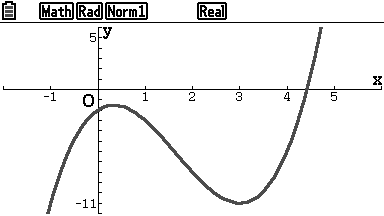
\includegraphics[scale=0.55]{assets/26-graph6.png}
          \end{vwcol}

          \begin{multicols}{2}
              \item $y = x^3 - 3x^2 + 4$
              \sol{}

              When $y = 0$,
              \begin{flalign*}
                  x^3 - 3x^2 + 4      & = 0               & \\
                  (x+1)(x^2 - 4x + 4) & = 0               & \\
                  (x+1)(x-2)^2        & = 0               & \\
                  x = -1              & \text{ or } x = 2
              \end{flalign*}
              $\therefore$ The $x$-intercepts are $(-1, 0)$ and $(2, 0)$.

              When $x = 0$, $y = 4$.

              $\therefore$ The $y$-intercept is $(0, 4)$.
              \begin{flalign*}
                  y'    & = 3x^2 - 6x       & \\
                  y''   & = 6x - 6          & \\
                  0     & = 3x^2 - 6x       & \\
                  0     & = x(x - 2)        & \\
                  x = 0 & \text{ or } x = 2
              \end{flalign*}
              When $x = 0$, $y'' = -6 < 0$.

              When $x = 2$, $y'' = 6 > 0$.

              $\therefore$ The function has a relative maximum point at $(0, 4)$ and a relative minimum point at $(2, 0)$.
              \begin{flalign*}
                  6x - 6 & = 0 & \\
                  x      & = 1
              \end{flalign*}
              When $x = 1$, $y = (1)^3 - 3(1)^2 + 4 = 2$.

              \noindent In the interval $(-\infty, 1)$, $y'' < 0$, hence the function is convex upward.

              \noindent In the interval $(1, \infty)$, $y'' > 0$, hence the function is convex downward.

              \noindent The point of inflection is $(1, 2)$.
              \vspace{2em}
              \begin{center}
                  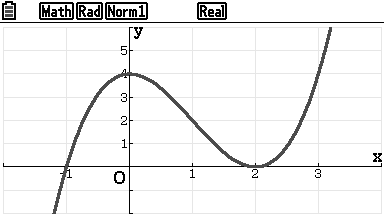
\includegraphics[scale=0.55]{assets/26-graph7.png}
              \end{center}
              \columnbreak

              \item In a container, the relationship between the volume of water $V$ (cm$^3$) and
              the depth of water $x$ (cm) is given by the equation $V = 4x^2 +
                  \dfrac{1}{6}x^3$. If the water is poured into the container at a rate of $6$
              cm$^3$ per second, find the rate of change of the depth of water when $x=2$ cm.
              \sol{}
              \begin{flalign*}
                  V              & = 4x^2 + \dfrac{1}{6}x^3                         & \\
                  \dfrac{dV}{dx} & = 8x + \dfrac{1}{2}x^2                           & \\
                  \dfrac{dV}{dt} & = 6                                              & \\
                  \dfrac{dx}{dt} & = \dfrac{dx}{dV} \cdot \dfrac{dV}{dt}            & \\
                                 & = \dfrac{1}{\dfrac{dV}{dx}} \cdot \dfrac{dV}{dt} & \\
                                 & = \dfrac{1}{8x + \dfrac{1}{2}x^2} \cdot 6        & \\
                                 & = \dfrac{6}{8x + \dfrac{1}{2}x^2}
              \end{flalign*}
              When $x = 2$,
              \begin{flalign*}
                  \dfrac{dx}{dt} & = \dfrac{6}{8(2) + \dfrac{1}{2}(2)^2} & \\
                                 & = \dfrac{6}{18}                       & \\
                                 & = \dfrac{1}{3} \text{ cm s}^{-1}
              \end{flalign*}
          \end{multicols}

          \newpage
    \item The water is poured into a conical pool with a height and a base radius of
          $20$m and $10$m respectively at a rate of $5$m$^3$/min. When the height of the
          water is $10$m, find
          \begin{enumerate}
              \item the rate of increasing of the height of the water. \sol{}

                    Let the height of the water be $h$cm and the radius of the water surface be
                    $r$cm.
                    \begin{flalign*}
                        \dfrac{h}{20}  & = \dfrac{r}{10}                                  & \\
                        r              & = \dfrac{h}{2}                                   & \\
                        V              & = \dfrac{1}{3}\pi r^2 h                          & \\
                                       & = \dfrac{1}{3}\pi \left(\dfrac{h}{2}\right)^2 h  & \\
                                       & = \dfrac{1}{12}\pi h^3                           & \\
                        \dfrac{dV}{dh} & = \dfrac{1}{4}\pi h^2                            & \\
                        \dfrac{dV}{dt} & = 5                                              & \\
                        \dfrac{dh}{dt} & = \dfrac{dh}{dV} \cdot \dfrac{dV}{dt}            & \\
                                       & = \dfrac{1}{\dfrac{dV}{dh}} \cdot \dfrac{dV}{dt} & \\
                                       & = \dfrac{1}{\dfrac{1}{4}\pi h^2} \cdot 5         & \\
                                       & = \dfrac{20}{\pi h^2} \text{ m min}^{-1}
                    \end{flalign*}
                    When $h = 10$,
                    \begin{flalign*}
                        \dfrac{dh}{dt} & = \dfrac{20}{\pi (10)^2}             & \\
                                       & = \dfrac{1}{5\pi} \text{ m min}^{-1}
                    \end{flalign*}

              \item the rate of change of the area of the water surface. \sol{}
                    \begin{flalign*}
                        A              & = \pi r^2                         & \\
                                       & = \pi \left(\dfrac{h}{2}\right)^2 & \\
                                       & = \dfrac{1}{4}\pi h^2             & \\
                        \dfrac{dA}{dh} & = \dfrac{1}{2}\pi h
                    \end{flalign*}
                    When $h = 10$,
                    \begin{flalign*}
                        \dfrac{dh}{dt} & = \dfrac{1}{5\pi}                            & \\
                        \dfrac{dA}{dt} & = \dfrac{dA}{dh} \cdot \dfrac{dh}{dt}        & \\
                                       & = \dfrac{1}{2}\pi (10) \cdot \dfrac{1}{5\pi} & \\
                                       & = 1 \text{ m}^2 \text{ min}^{-1}
                    \end{flalign*}
          \end{enumerate}

    \item The radius of a spherical container decreases from $4$cm to $3.95$cm. Find the
          approximate amount of decrease in the volume and the surface area of the
          container. \sol{}
          \begin{flalign*}
              V                          & = \dfrac{4}{3}\pi r^3     & \\
              A                          & = 4\pi r^2                & \\
              \dfrac{dV}{dr}             & = 4\pi r^2                & \\
              \dfrac{dA}{dr}             & = 8\pi r                  & \\
              \dfrac{\Delta V}{\Delta r} & = \dfrac{dV}{dr}          & \\
              \Delta V                   & = 4\pi r^2 \cdot \Delta r & \\
              \dfrac{\Delta A}{\Delta r} & = \dfrac{dA}{dr}          & \\
              \Delta A                   & = 8\pi r \cdot \Delta r
          \end{flalign*}
          When $r = 4$,$\Delta r = -0.05$,
          \begin{flalign*}
              \Delta V & = 4\pi (4)^2 (-0.05)   & \\
                       & = -3.2\pi \text{ cm}^3 & \\
              \Delta A & = 8\pi (4)(-0.05)      & \\
                       & = -1.6\pi \text{ cm}^2
          \end{flalign*}
          $\therefore$ The approximate amount of decrease in the volume and the surface area of the container is $-3.2\pi$cm$^3$ and $-1.6\pi$cm$^2$ respectively.
          \vfill\null

    \item The capacity of water of a spherical container is given by $V =
              \left[\dfrac{\pi h^2}{3}(15-h)\right]$cm$^3$, where $h$ is the depth of the
          water. Find the approximate amount of increase in the capacity of the container
          when the depth of the water increases from $4$cm to $4.01$cm. \sol{}
          \begin{flalign*}
              V                          & = 5\pi h^2 - \dfrac{1}{3}\pi h^3     & \\
              \dfrac{dV}{dh}             & = 10\pi h - \pi h^2                  & \\
              \dfrac{\Delta V}{\Delta h} & = \dfrac{dV}{dh}                     & \\
              \Delta V                   & = (10\pi h - \pi h^2) \cdot \Delta h &
          \end{flalign*}
          When $h = 4$,$\Delta h = 0.01$,
          \begin{flalign*}
              \Delta V & = (10\pi (4) - \pi (4)^2) \cdot 0.01 & \\
                       & = 0.24\pi \text{ cm}^3
          \end{flalign*}
          $\therefore$ The approximate amount of increase in the capacity of the container is $0.24\pi$cm$^3$.
          \vfill\null

          \newpage

    \item In a bowl, when the height of the water is $h$cm, the volume of the water is
          given by $V = \left(h^3 + 3h^2 + 11h\right)$cm$^3$. When the height of the
          water is $7cm$, pour an additional $\Delta V$cm$^3$ of water into the bowl.
          Find the approximate amount of increase in the height of the water. \sol{}
          \begin{flalign*}
              \dfrac{dV}{dh}             & = 3h^2 + 6h + 11                   & \\
              \dfrac{\Delta V}{\Delta h} & = \dfrac{dV}{dh}                   & \\
              \Delta V                   & = (3h^2 + 6h + 11) \cdot \Delta h  & \\
              \Delta h                   & = \dfrac{\Delta V}{3h^2 + 6h + 11}
          \end{flalign*}
          When $h = 7$,
          \begin{flalign*}
              \Delta h & = \dfrac{\Delta V}{3(7)^2 + 6(7) + 11} & \\
                       & = \dfrac{\Delta V}{200} \text{ cm}
          \end{flalign*}
          $\therefore$ The approximate amount of increase in the height of the water is $\dfrac{\Delta V}{200}$cm.

    \item If $y = \dfrac{1}{\sqrt[3]{x}}$, find $\dfrac{dy}{dx}$. Hence, find the
          approximate value of $\dfrac{1} {\sqrt[3]{130}}$. (Correct to 3 decimal places)
          \sol{}
          \begin{flalign*}
              y                          & = x^{-\frac{1}{3}}                             & \\
              \dfrac{dy}{dx}             & = -\dfrac{1}{3}x^{-\frac{4}{3}}                & \\
              \dfrac{\Delta y}{\Delta x} & = \dfrac{dy}{dx}                               & \\
              \Delta y                   & = -\dfrac{1}{3}x^{-\frac{4}{3}} \cdot \Delta x
          \end{flalign*}
          When $x = 125$, $\Delta x = 5$,
          \begin{flalign*}
              \Delta y & = -\dfrac{1}{3}(125)^{-\frac{4}{3}} \cdot 5 & \\
                       & = -0.003
          \end{flalign*}
          $\therefore$ The approximate value of $\dfrac{1} {\sqrt[3]{130}}$ is $\dfrac{1}{5} - 0.003 = 0.197$.
\end{enumerate}
